%!TEX program = xelatex
\documentclass{beamer}
%\documentclass[aspectratio=169]{beamer} %如果需要16:9
\usepackage{ctex}
\usepackage{times}
\usepackage{multicol}
\usepackage{multirow}
\usetheme{Warsaw}
\usepackage{tikz}
\usetikzlibrary{arrows,shapes,chains}
\usepackage[super,square]{natbib}
\usepackage{tabularx}
\usepackage{booktabs}
\usepackage{longtable}
\usepackage{graphicx}
%\usecolortheme{beaver}     % use white-grey colour style
%\beamersetaveragebackground{black!10}
% This is only inserted into the PDF information catalog. Can be left out.
\subject{presentation}
\keywords{example}
\useinnertheme{circles}%{rectangles}
\setbeamertemplate{itemize item}{$\circledast$}%{\checkmark}

%% ======================================================
%%     preamble
%% ======================================================
\title{基于SpringMVC架构WEB应用系统优化研究}
\author{答辩人:武斌}
\institute
{
  导师:郑海永\\
  电子系~中国海洋大学
  \and
   Department electronic engineering \\
  Ocean University Of China
}
% \date{\today}
\date{2017年5月25日}

\logo{
\includegraphics[height=0.09\textwidth]{./logo/Ocean_University_of_China.png}}


%% ======================================================
\begin{document}

%% ++++++++++++++++++++++++++++++++++++++++++++++++++++++
%% title page
%% ++++++++++++++++++++++++++++++++++++++++++++++++++++++
\begin{frame}
  \titlepage
\end{frame}

%% ++++++++++++++++++++++++++++++++++++++++++++++++++++++
%%     目录
%% ++++++++++++++++++++++++++++++++++++++++++++++++++++++
%\section{概述}
\begin{frame}
  \frametitle{目录}
  \begin{enumerate}
    \item<1-> 题目来源及目的
    \item<1-> 研究方法及内容
    \item<1-> 研究结论及展望
  \end{enumerate}
\end{frame}


%% ++++++++++++++++++++++++++++++++++++++++++++++++++++++
%%      正文
%% ++++++++++++++++++++++++++++++++++++++++++++++++++++++
%% ++++++++++++++++++++++++++++++++++++++++++++++++++++++
%%      选题背景
%% ++++++++++++++++++++++++++++++++++++++++++++++++++++++
%\section{选题来源和背景分析 }
%\subsection{系统结构}
\begin{frame}
  \frametitle{来源及目的}
  \begin{block}{题目来源}
  	\begin{itemize}
  		\item 本人在海信参与的项目,负责DevOps的研究和实践,目的是实现产品的持续交付和快速部署。
  		% \item 目前的参考文献中很少有针对于单一系统的整体性优化策略研究;
  	\end{itemize}
  \end{block}
  \begin{block}{研究目的}
  	\begin{itemize}
  		\item 研究系统开发过程中的代码交付、持续集成、服务器运维等方面的优化策略
      \item 基于现有的WEB项目研究一种切实可用的WEB平台开发运维优化方案,为有相同需求的研发人员提供借鉴和参考
  	\end{itemize}
  \end{block}
\end{frame}
%% ++++++++++++++++++++++++++++++++++++++++++++++++++++++
%%      研究内容
%% ++++++++++++++++++++++++++++++++++++++++++++++++++++++
\begin{frame}
  \frametitle{方法及内容}
  \begin{enumerate}
    \item<1-> 研究的基本框架
    \item<1-> 应用性能优化
    \item<1-> 数据库性能优化
    \item<1-> 服务器稳定性优化
  \end{enumerate}
\end{frame}

\begin{frame}
  \frametitle{平台开发基本框架}
  \begin{figure}
  \centering
    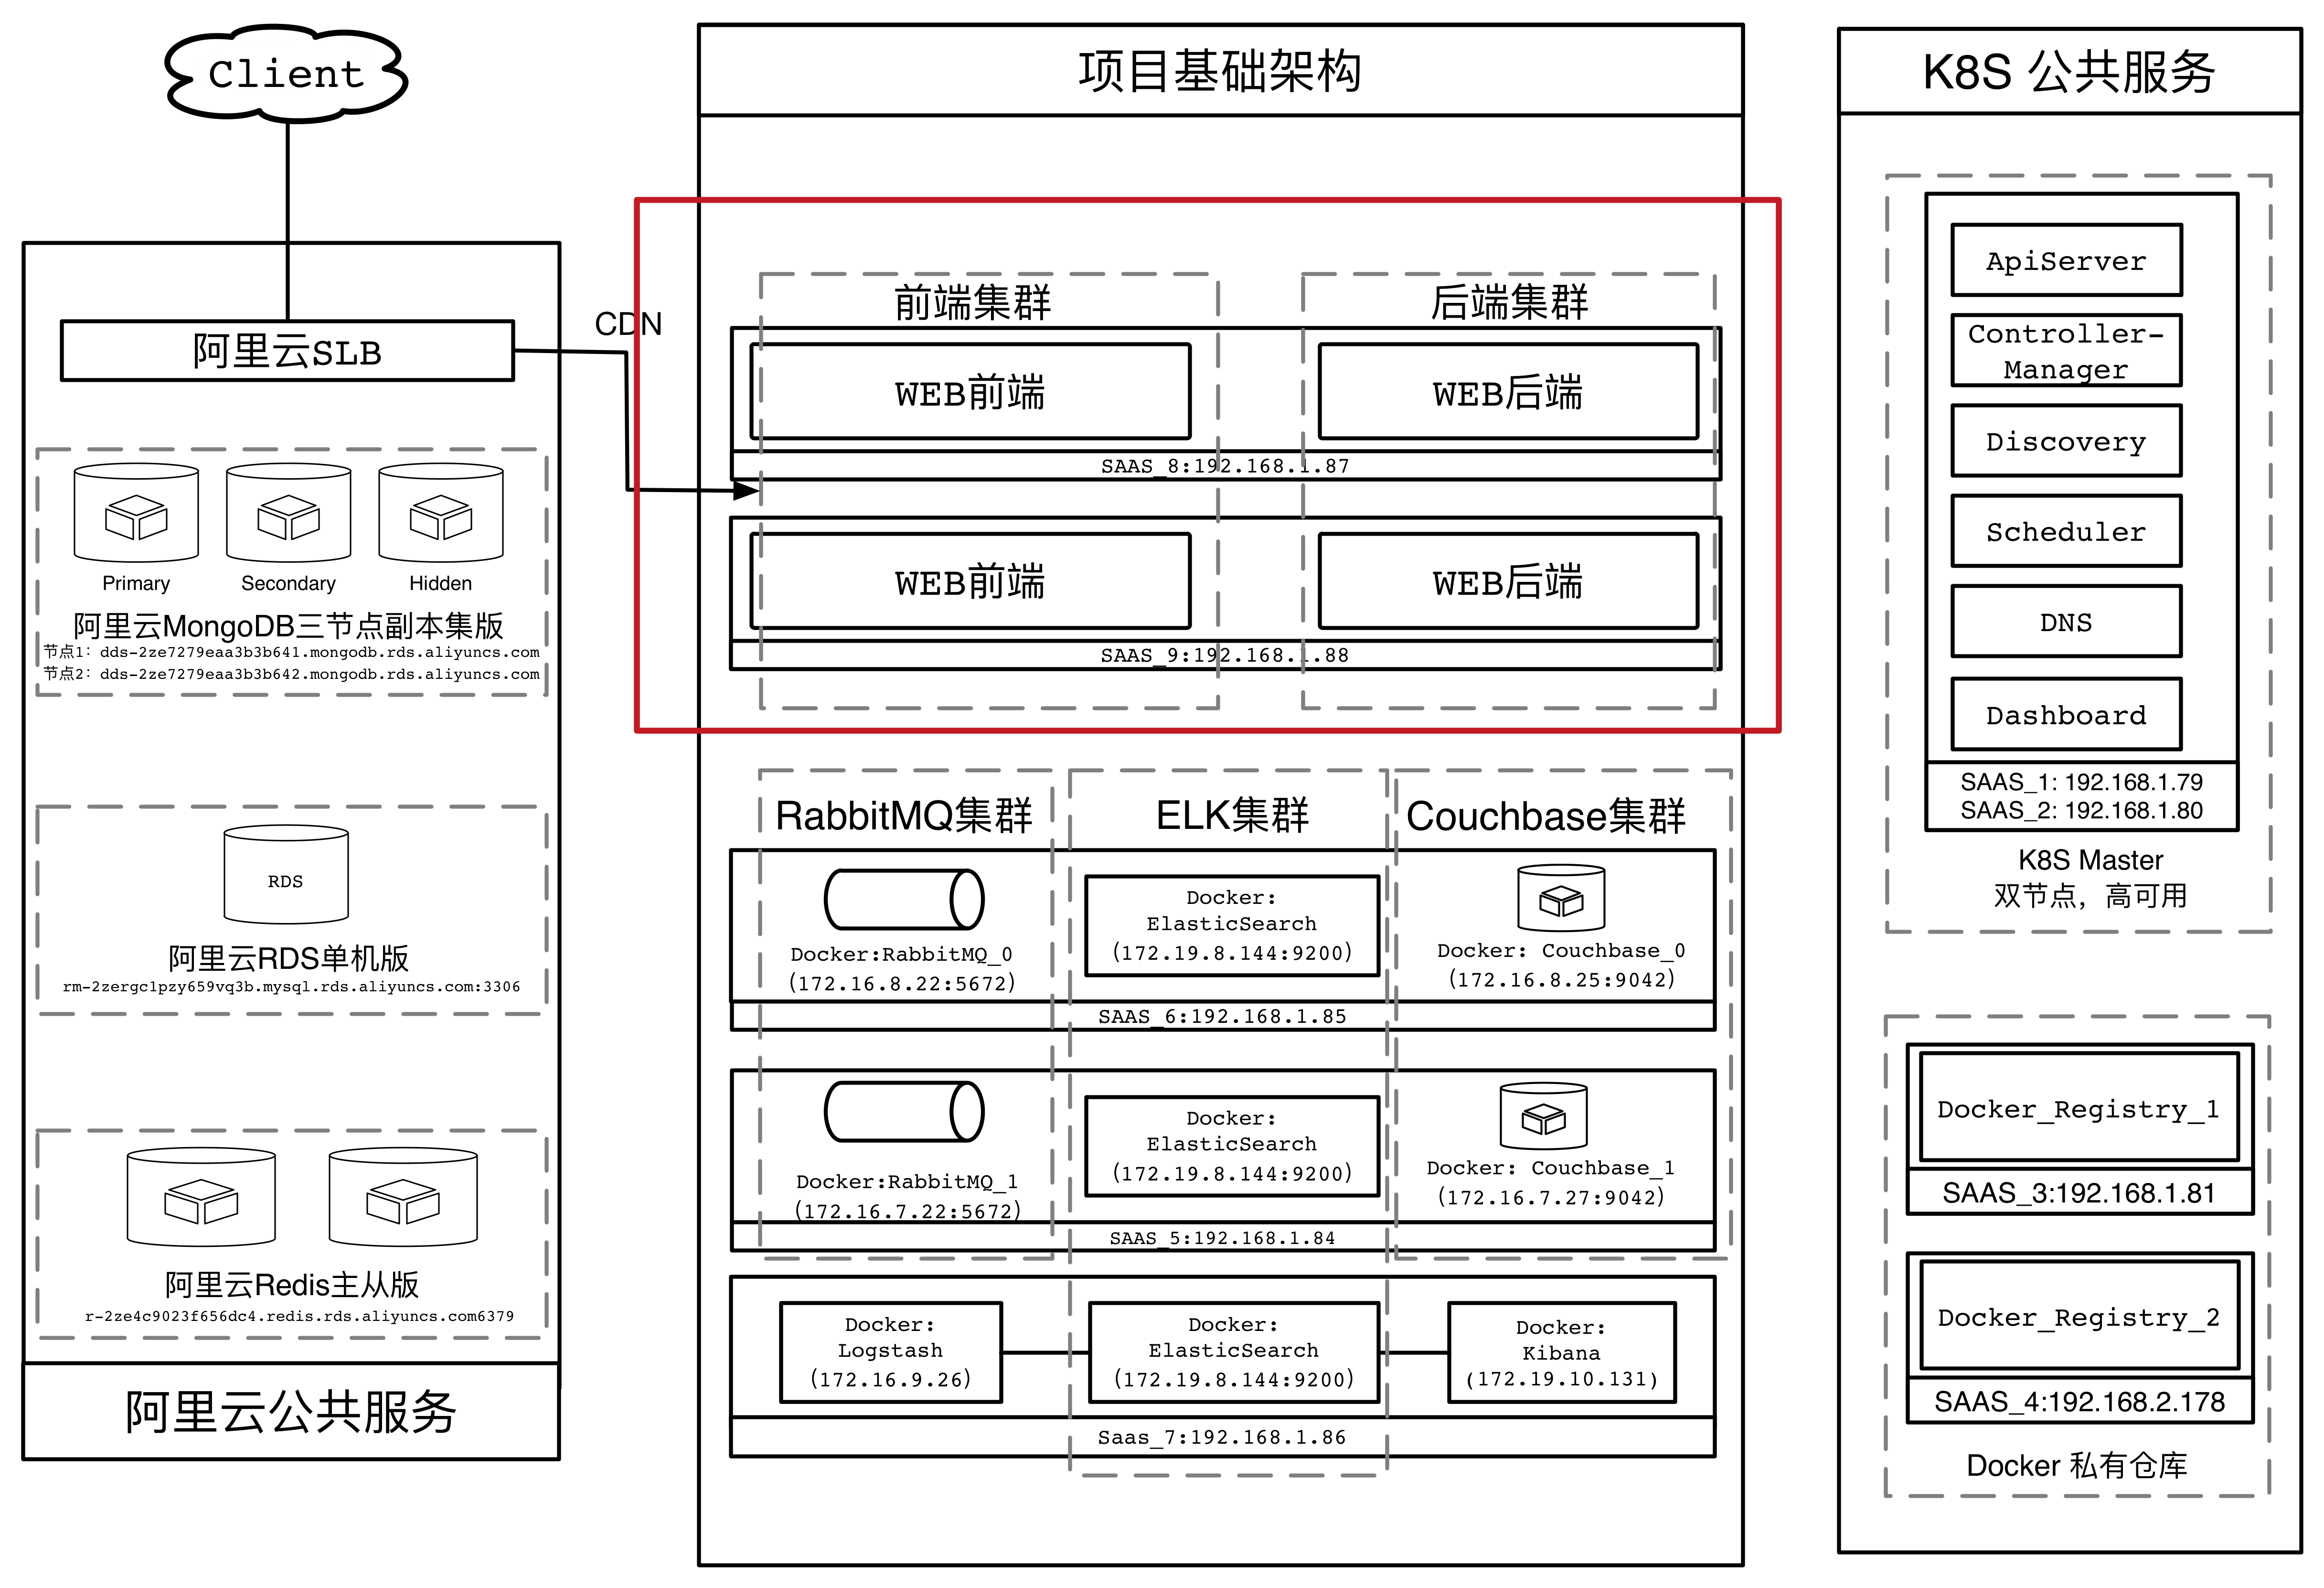
\includegraphics[width=\textwidth]{./img/02/deploy.png}
    % \caption{平台开发基本框架}
    \label{fig:deploy}
  \end{figure}
\end{frame}

\begin{frame}
  \frametitle{研究的主要内容}
  \begin{figure}
  \centering
    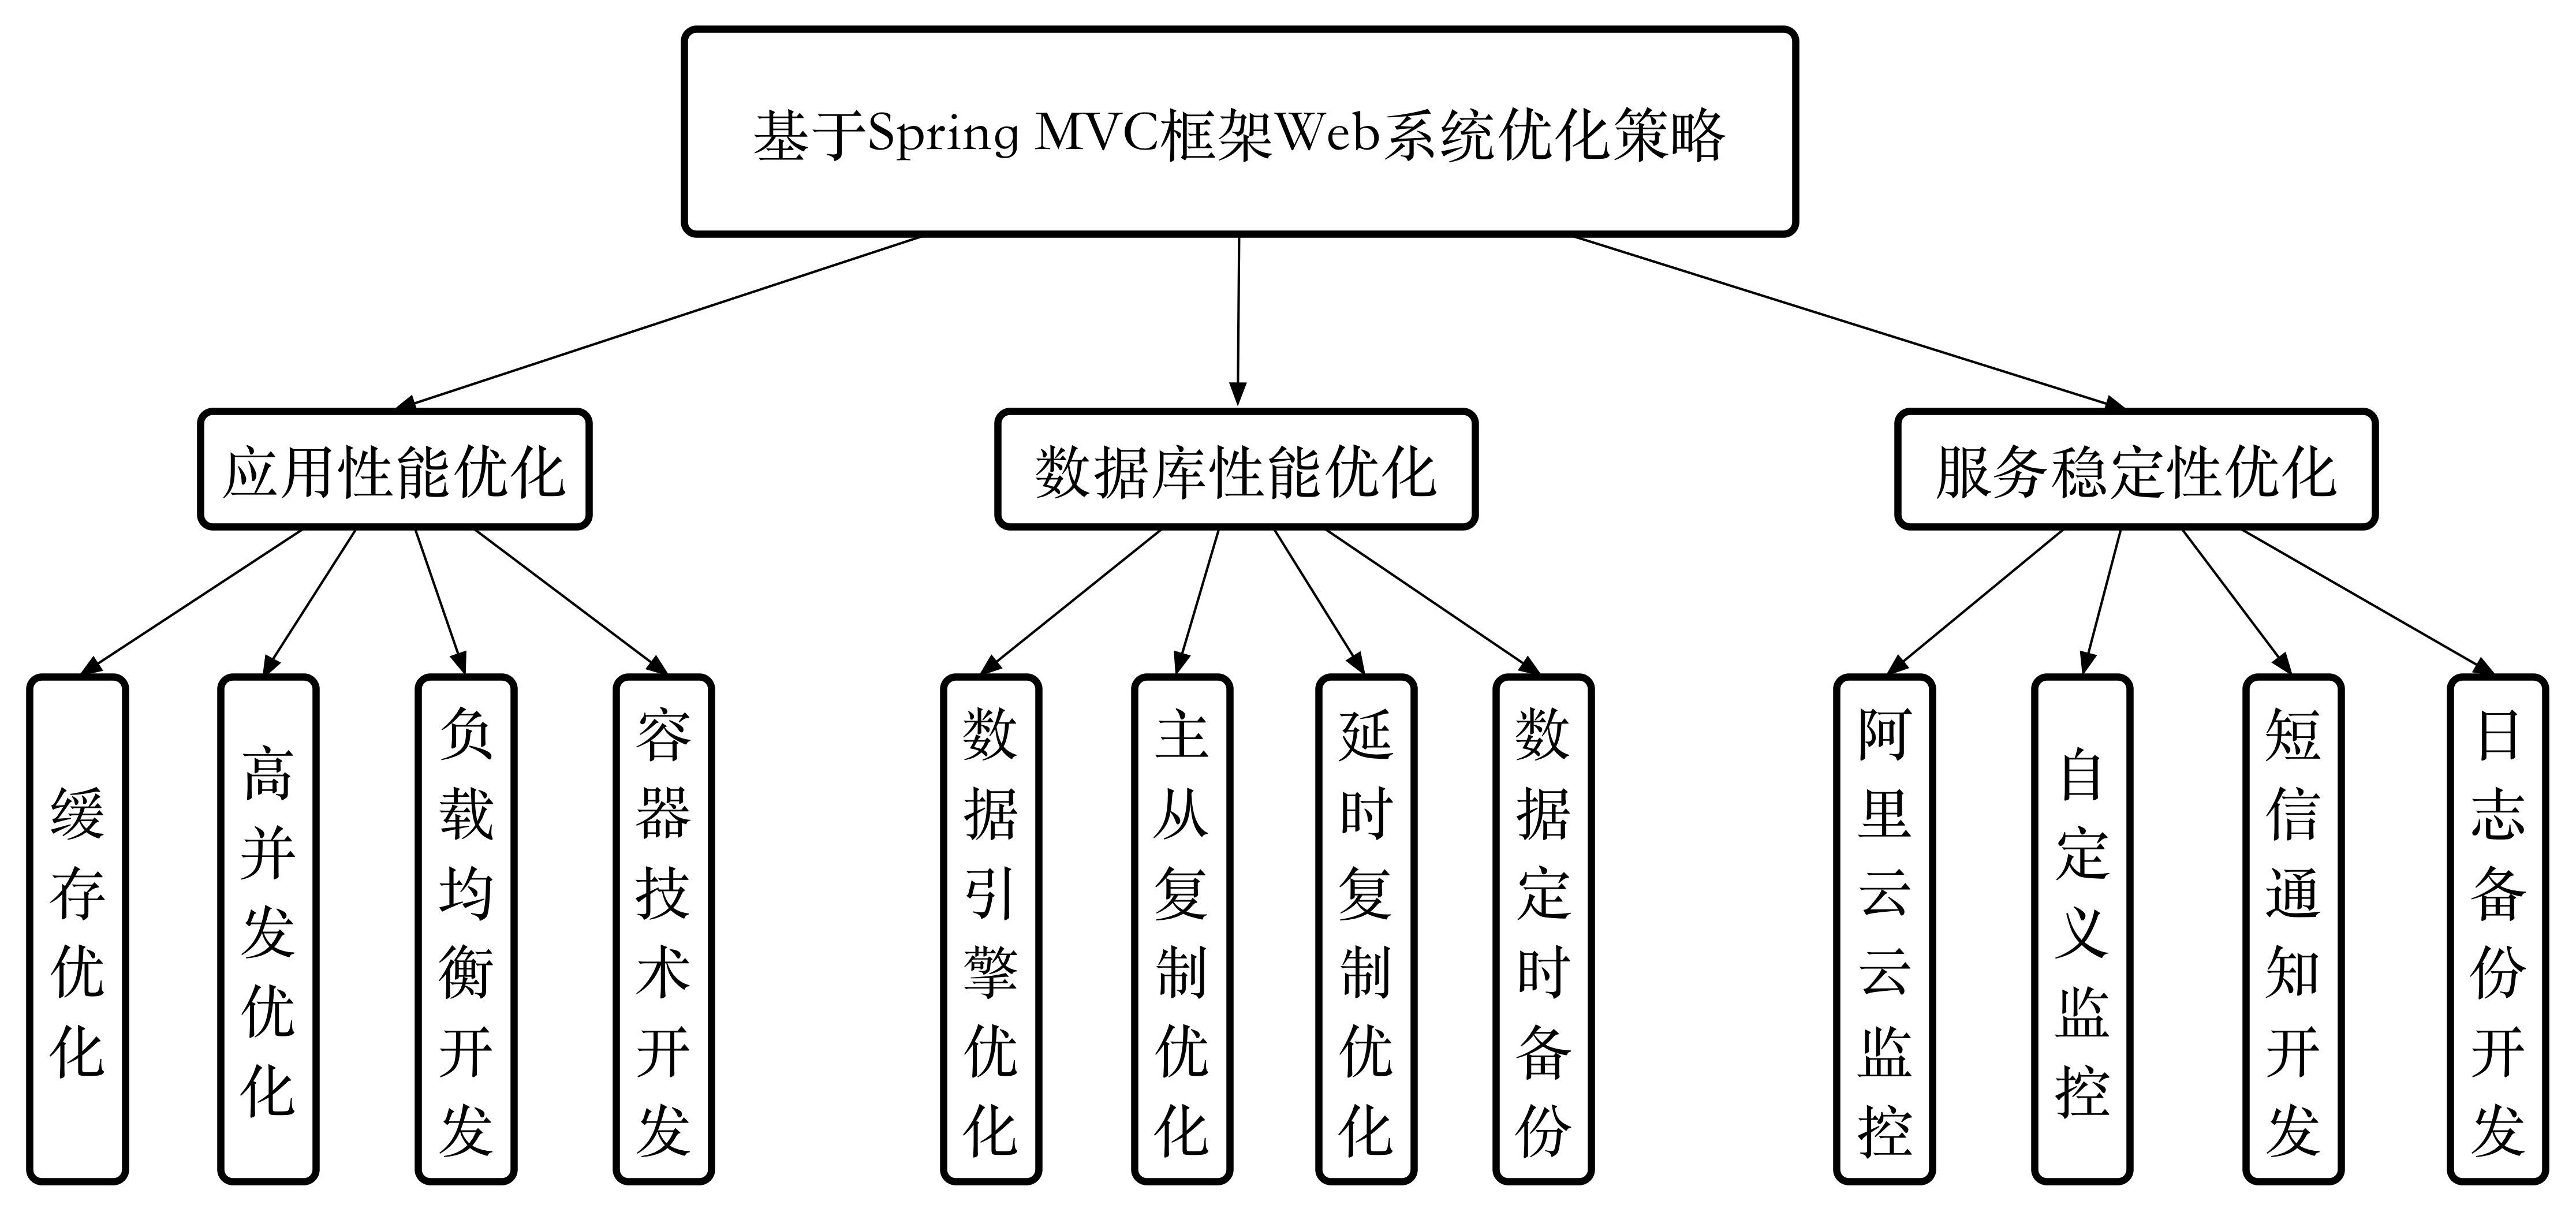
\includegraphics[height=5cm]{./img/02/summery.png}
    \caption{平台功能}
    \label{fig:summery}
  \end{figure}
\end{frame}

\begin{frame}
  \frametitle{一、应用性能优化}
    \begin{block}{1. Couchbase缓存优化}
      \begin{itemize}
        \item 将项目的基础数据在首次访问时加载到缓存中
      \end{itemize}
    \end{block}
    \begin{columns}
      \begin{column}{0.40\textwidth}
        \rightline{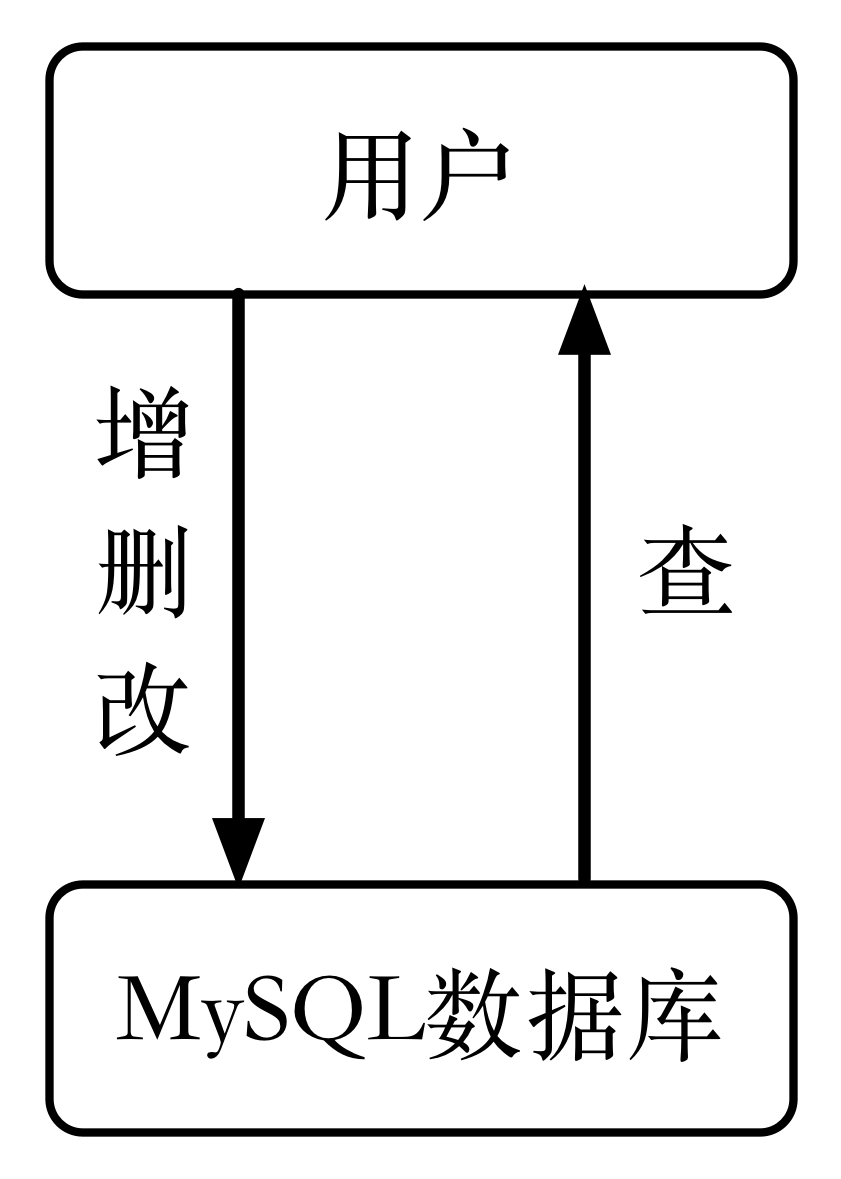
\includegraphics[height=3.5cm]{./img/02/couchbase1.png}}
      \end{column}
      \begin{column}{0.20\textwidth}
        \centering
        
\includegraphics[width=2cm]{./img/02/arrow.png}
        \label{fig:arrow}
      \end{column}
      \begin{column}{0.40\textwidth}
        \leftline{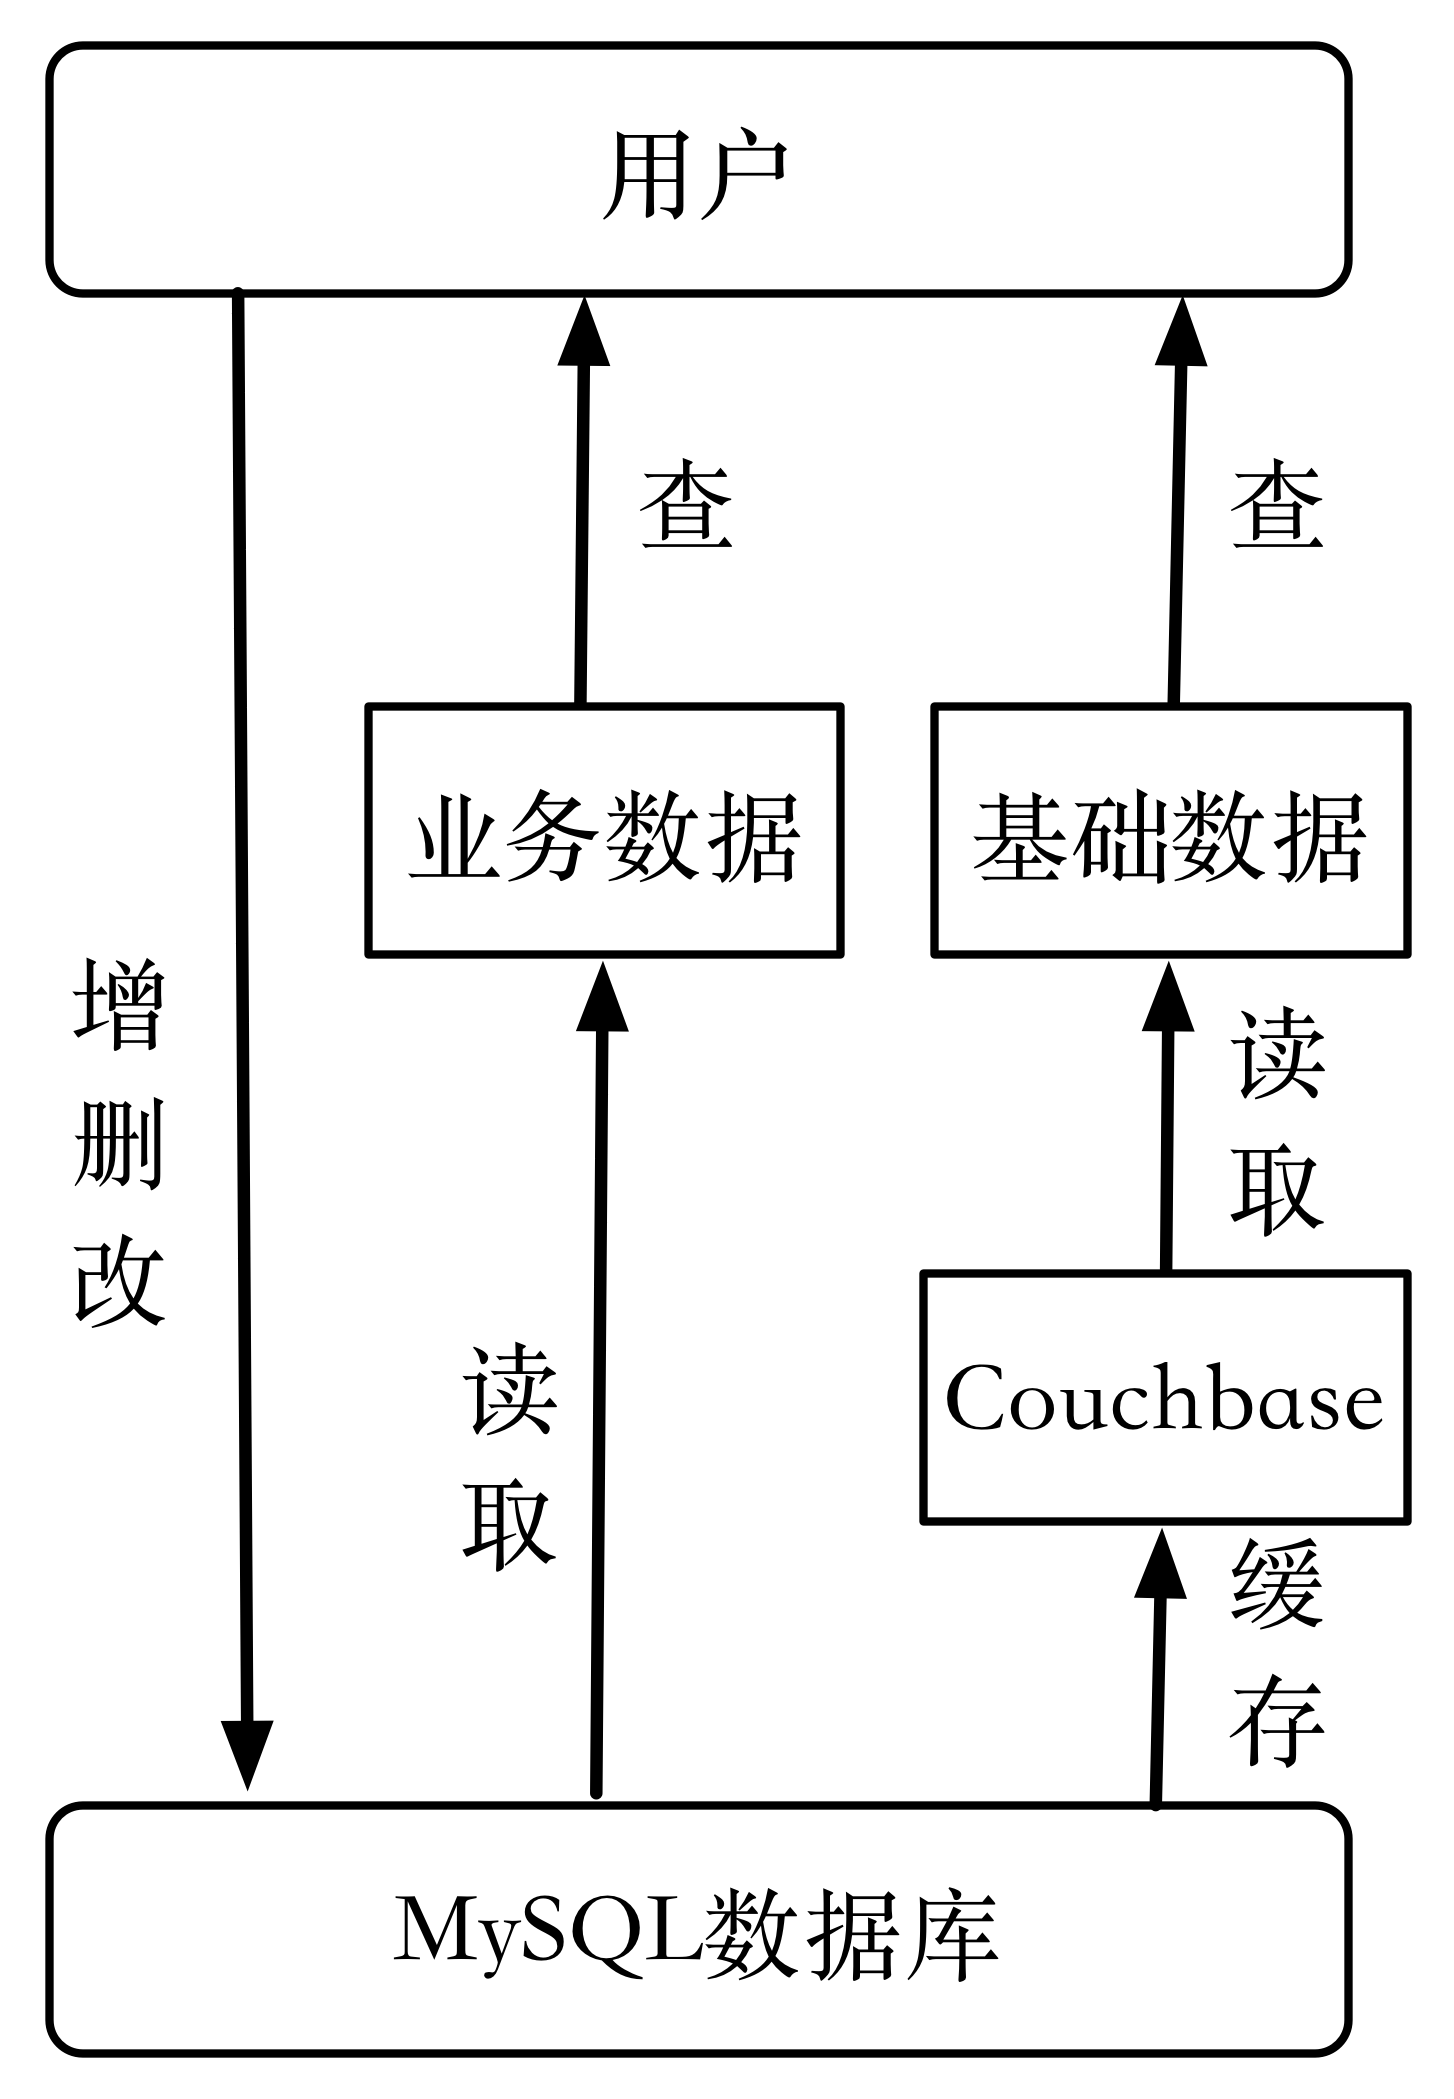
\includegraphics[height=3.5cm]{./img/02/couchbase2.png}}
      \end{column}
    \end{columns}
    \begin{table}[htb]
    \centering
    \begin{minipage}[t]{\linewidth} % 如果想在表格中使用脚注,minipage是个不错的办法
    \centering
    \scalebox{0.7}[0.7]{
    \label{tab:couchbase-test}
      \begin{tabularx}{\linewidth}{lXX}
        \toprule[1.5pt]
        {\heiti 测试参数} & {\heiti 关闭Couchbase} & {\heiti 开启Couchbase} \\\midrule[1pt]
        单次请求用时  &  0.670(s) & 0.113(s)\\
        请求失败次数 &  82 & 7 \\
        \bottomrule[1.5pt]
      \end{tabularx}
    }
    \end{minipage}
    \scalebox{0.7}[0.7]{\footnotesize{{ }{ }注: 10W次请求,每次100个并发}}
    \end{table}
\end{frame}

\begin{frame}
  \frametitle{一、应用性能优化}
    \begin{block}{2. Tomcat高并发APR优化}
      \footnotesize{
      Tomcat 节约用户高并发的处理方式有NIO和APR两种方式:
      \begin{itemize}
        \item NIO 模式是一 个基于缓冲区、并能提供非阻塞 I/O 操作的 Java API
        \item APR模式是从操作系统级别解决异步IO问题,大幅度的提高服务器的处理和响应性能,是Tomcat 运行高并发应用的首选模式。
      \end{itemize}
      }
    \end{block}
    \begin{table}[htb]
      \centering
      \begin{minipage}[t]{0.8\linewidth} % 如果想在表格中使用脚注,minipage是个不错的办法
      \scalebox{0.85}[0.85]{
      \label{tab:tomcat-apr}
        \begin{tabularx}{\linewidth}{lXXX}
          \toprule[1.5pt]
          {\heiti 请求次数} & {\heiti 并发数量} & {\heiti APR模式} &  {\heiti NIO模式}\\
          \midrule[1pt]
          10000&10 &6612.60&8255.48\\
          50000  &  10 & 7480.96 & 8841.41 \\
          100000  &  10 & 6588.83 & 8355.85 \\
          10000  &  1000 & 6966.93 & 6155.21 \\
          50000  &  1000 & 9187.63 & 1957.35 \\
          100000  &  1000 & 7751.47 & - \\
          \bottomrule[1.5pt]
        \end{tabularx}
        }
      \end{minipage}
    \end{table}
\end{frame}

\begin{frame}
  \frametitle{一、应用性能优化}
    \begin{block}{3. 容器化开发部署优化优化}
      \footnotesize 随着业务扩展,节点的快速部署和服务交付是性能优化过程中的重要工作。
    \end{block}
    \centering
    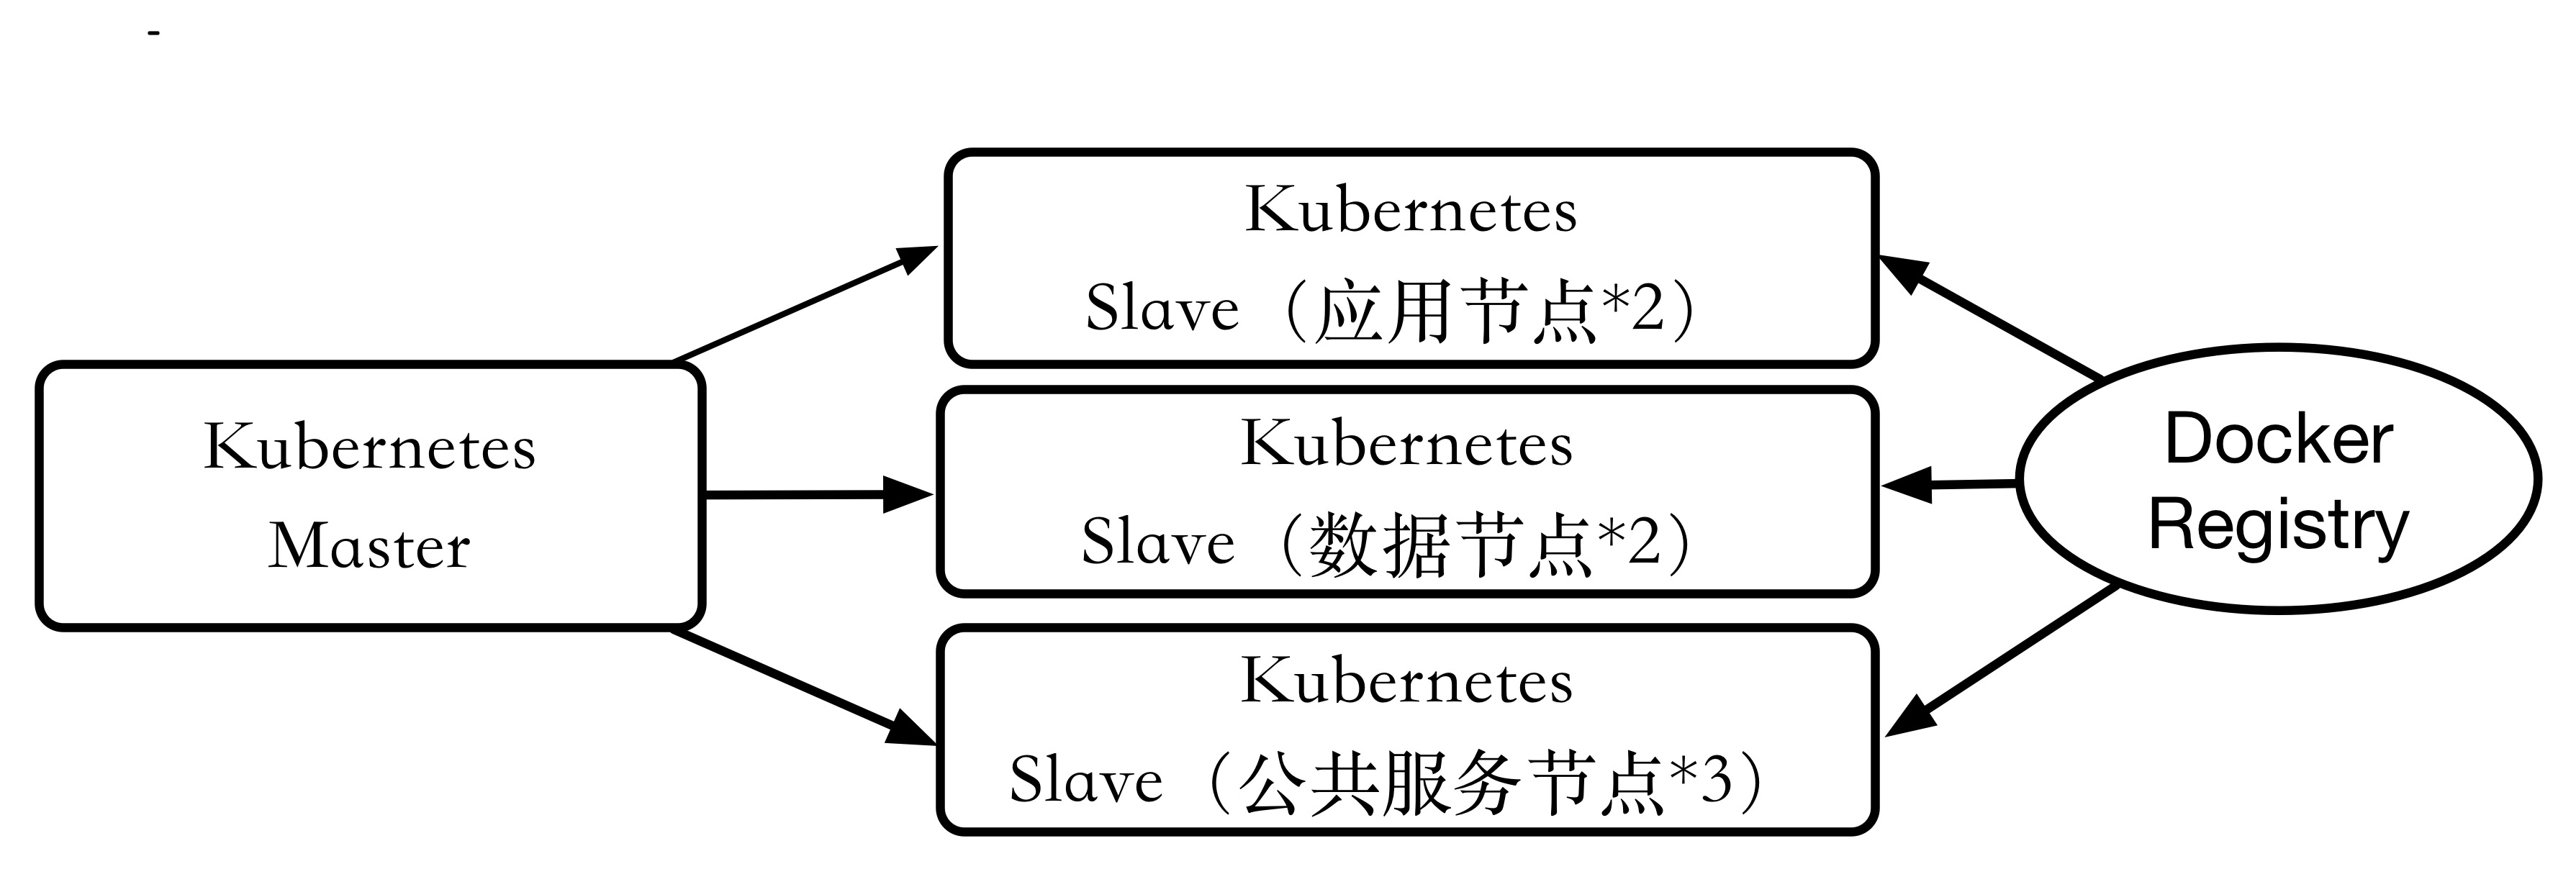
\includegraphics[height=3.5cm]{./img/k8scluster.png} \\
    \centering
    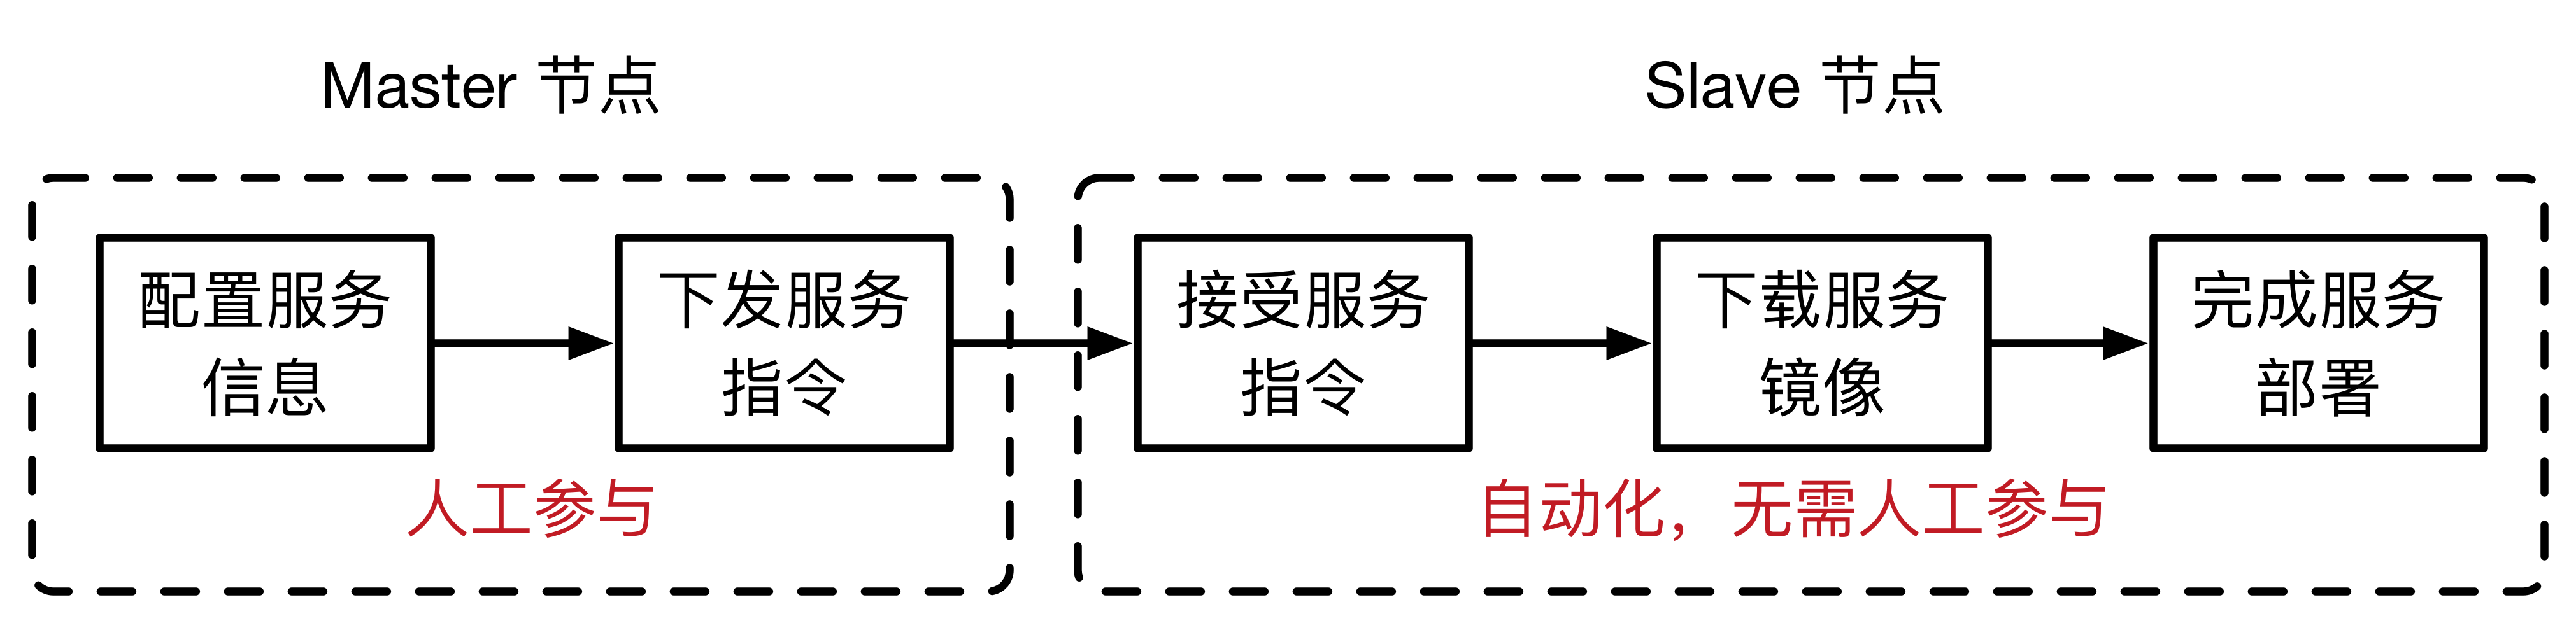
\includegraphics[height=2.5cm]{./img/k8sdeploy.png}\\
    \footnotesize 一次部署三个服务的时间在30秒,传统部署方式平均时间在15分钟左右。
\end{frame}

\begin{frame}
\frametitle{二、数据库性能优化}
  \begin{block}{数据库复制结构开发}
    对于商业平台而已,保证数据的实时性和数据备份是应用优化的一个主要部分。
  \end{block}
  \begin{columns}
    \begin{column}{0.50\textwidth}
      \centering
      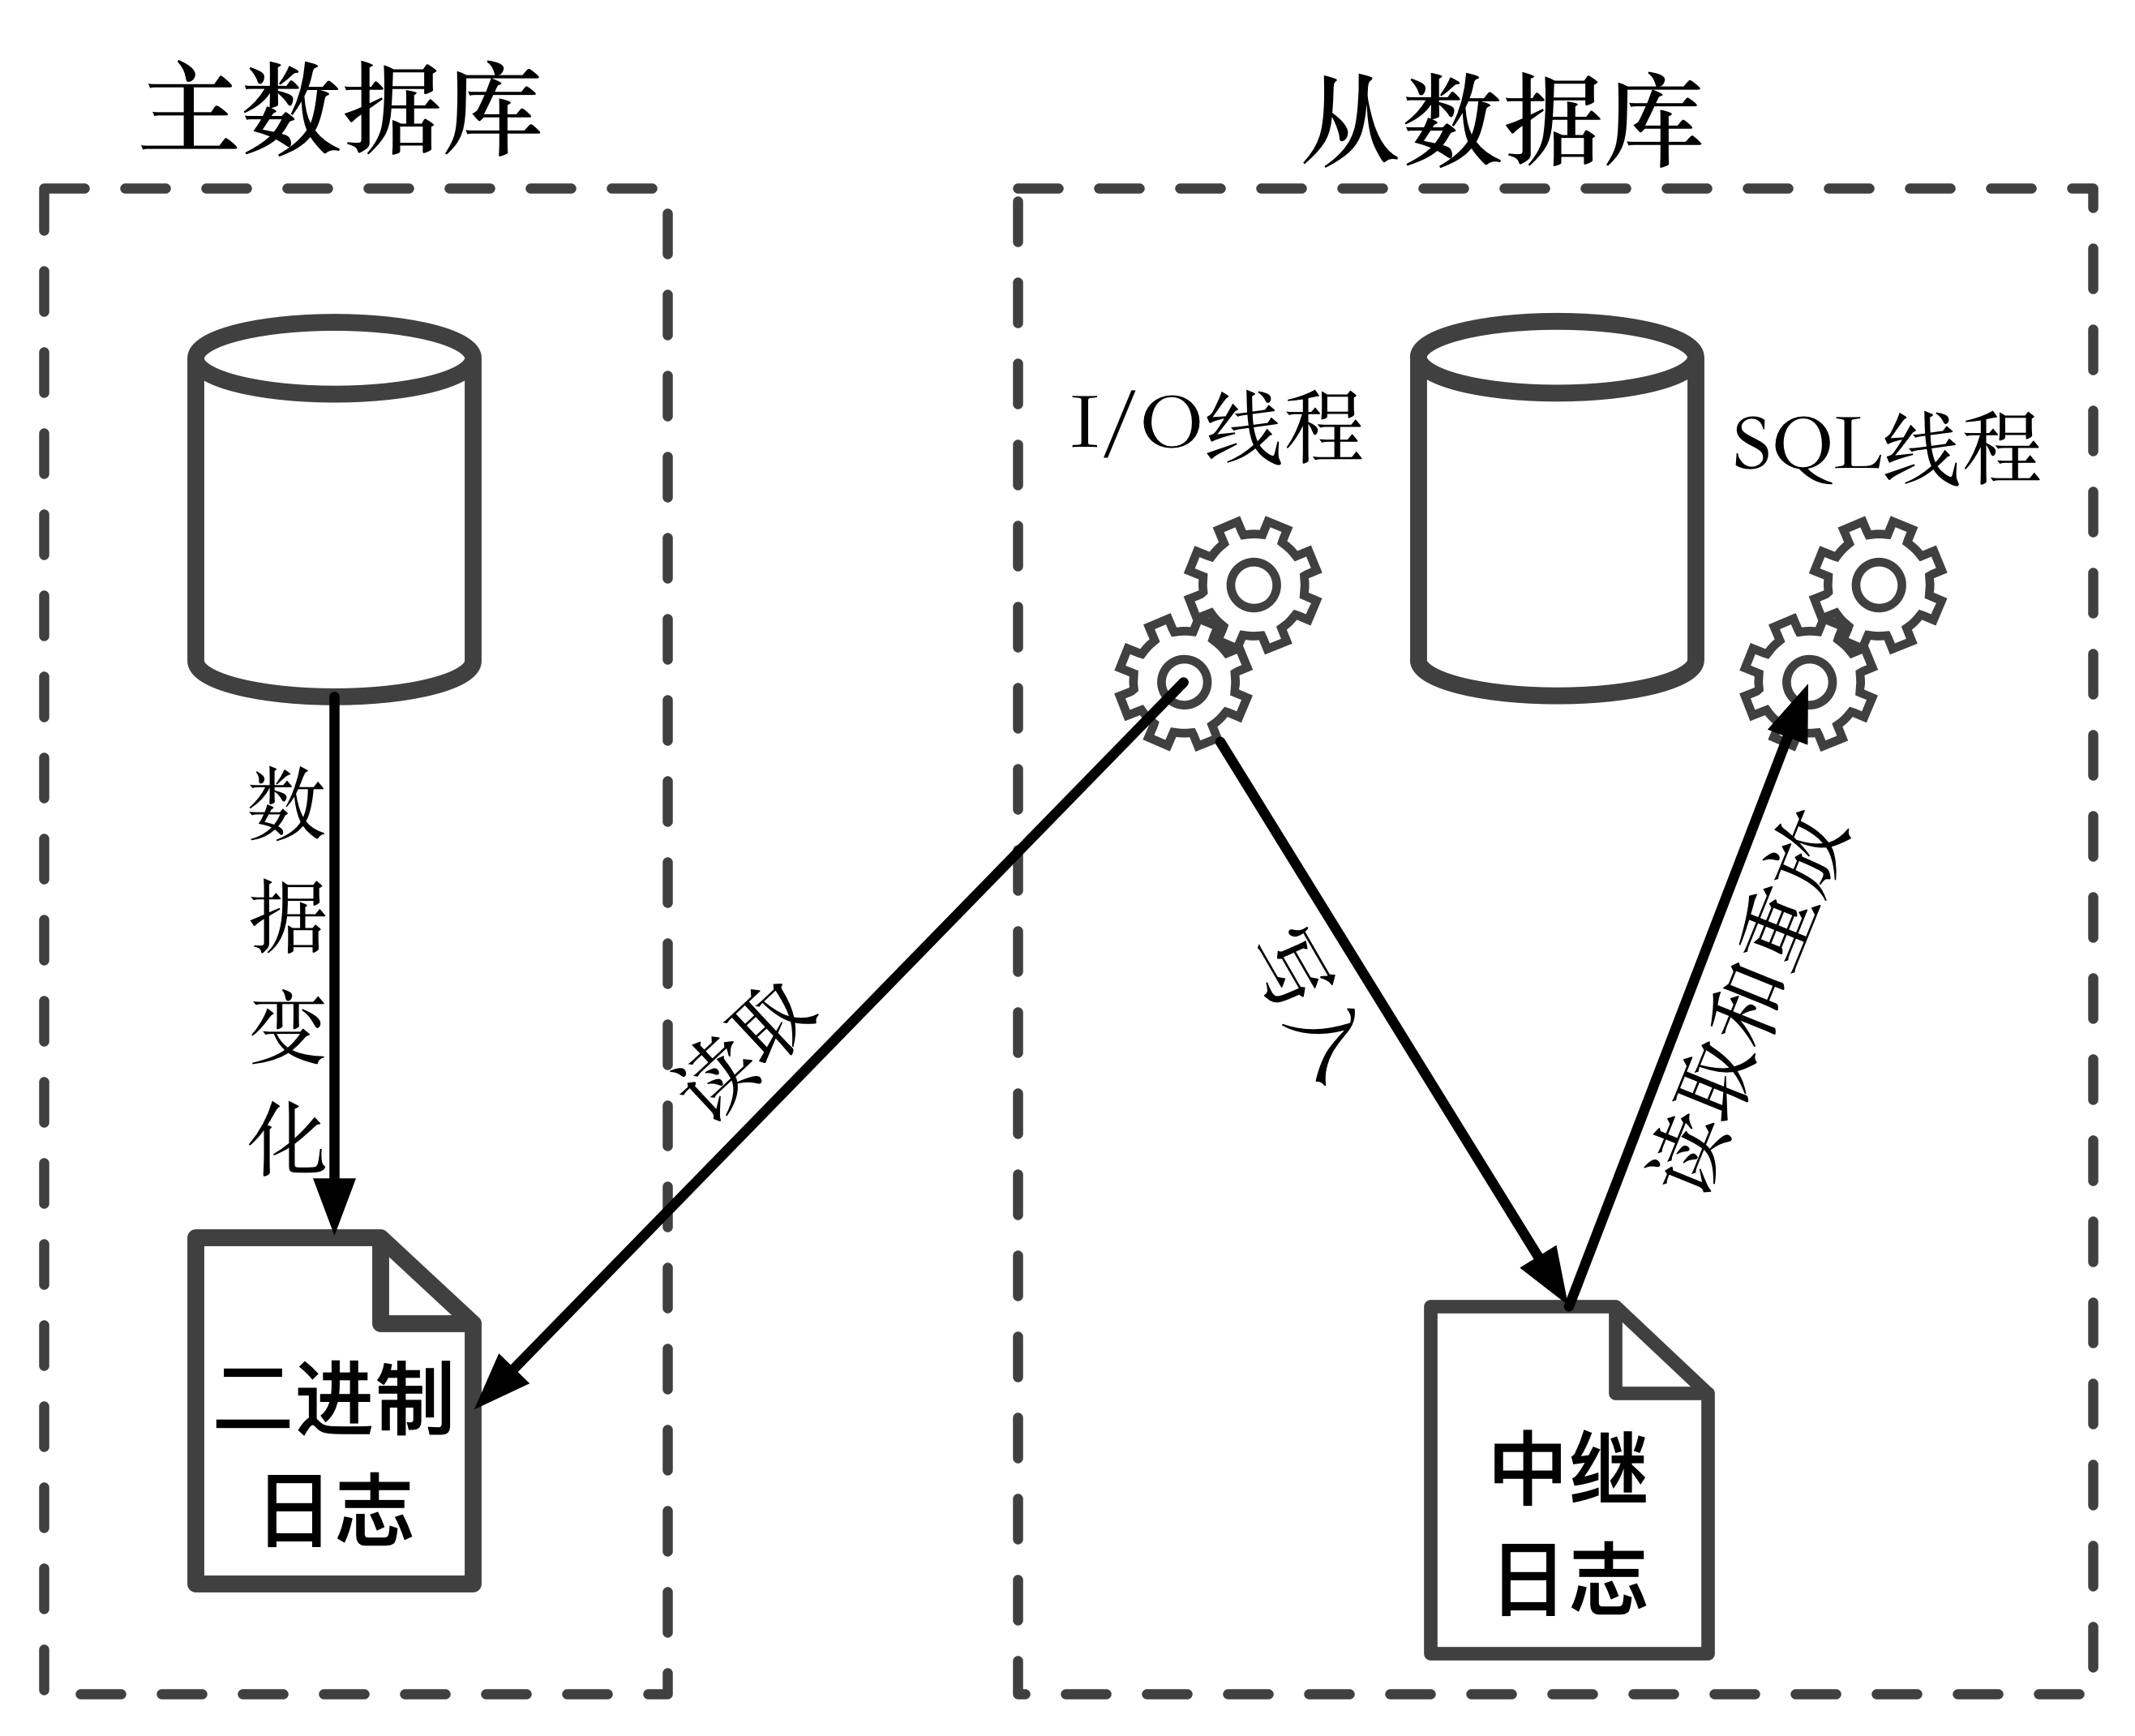
\includegraphics[width=5cm]{./img/03/sql.png}
      % \caption{docker容器架构}
      \label{fig:docker}
    \end{column}
    \begin{column}{0.50\textwidth}
      \centering
      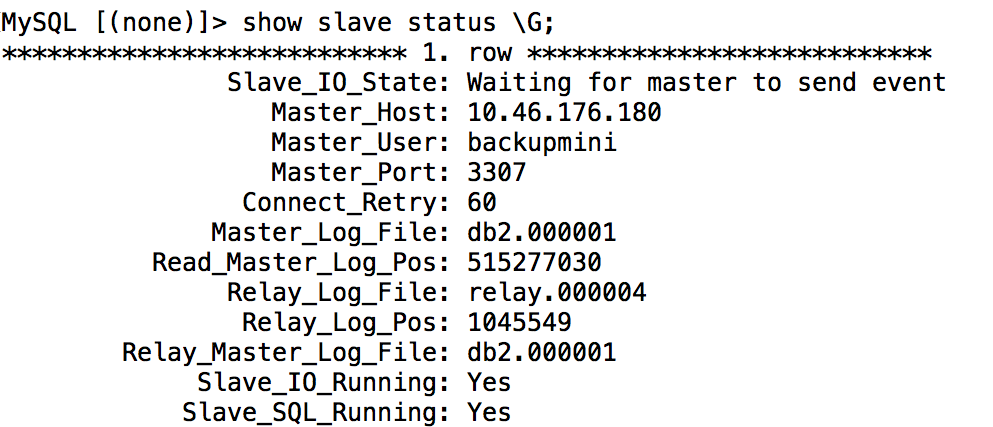
\includegraphics[width=6cm]{./img/mysqlstatus.png}
    \end{column}
  \end{columns}
  \centering
  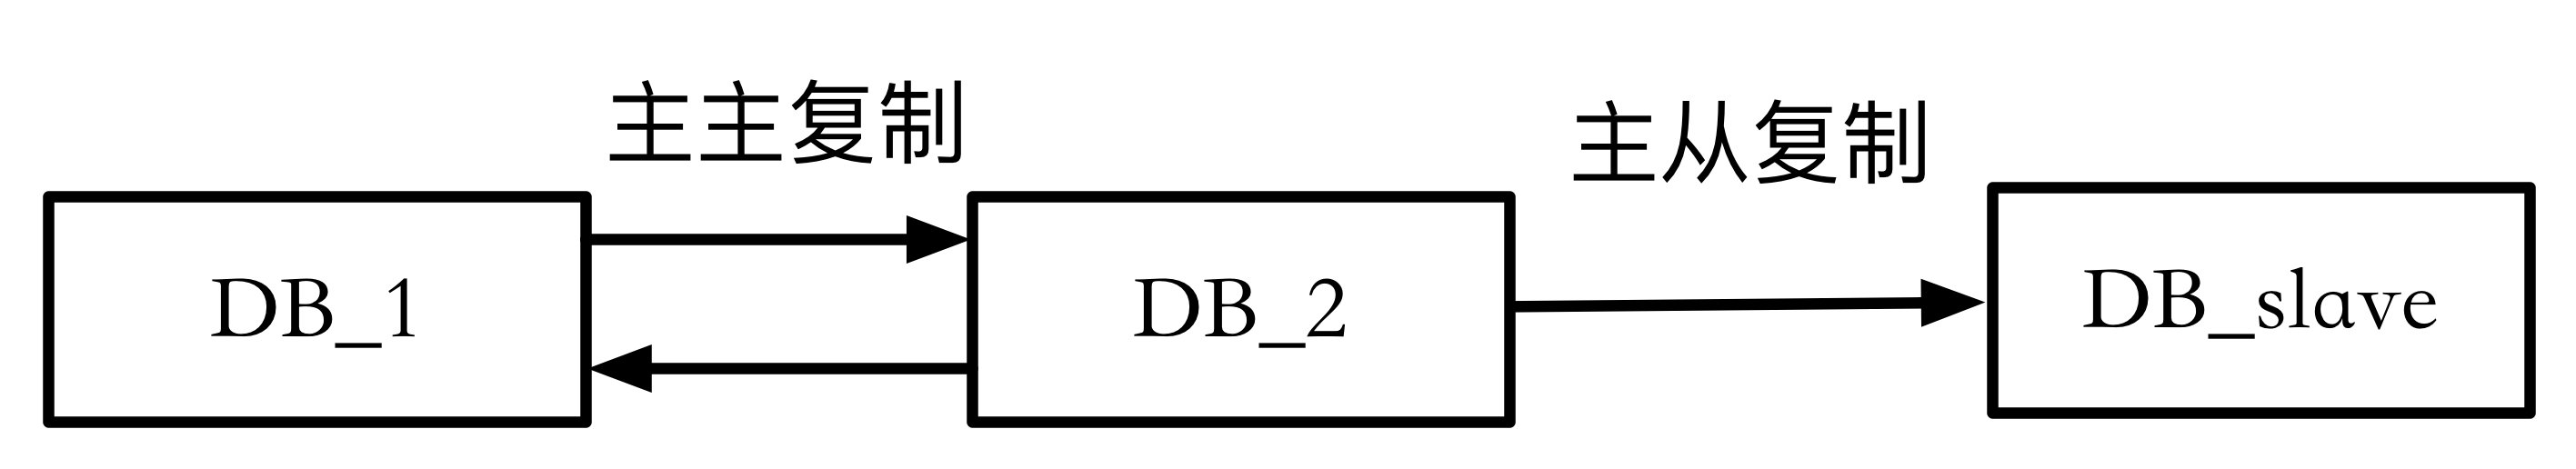
\includegraphics[width=8cm]{./img/mysqlcluster.png}
\end{frame}

\begin{frame}
\frametitle{三、服务器稳定性优化}
  \begin{columns}
    \begin{column}{0.60\textwidth}
      \begin{figure}
      \centering
        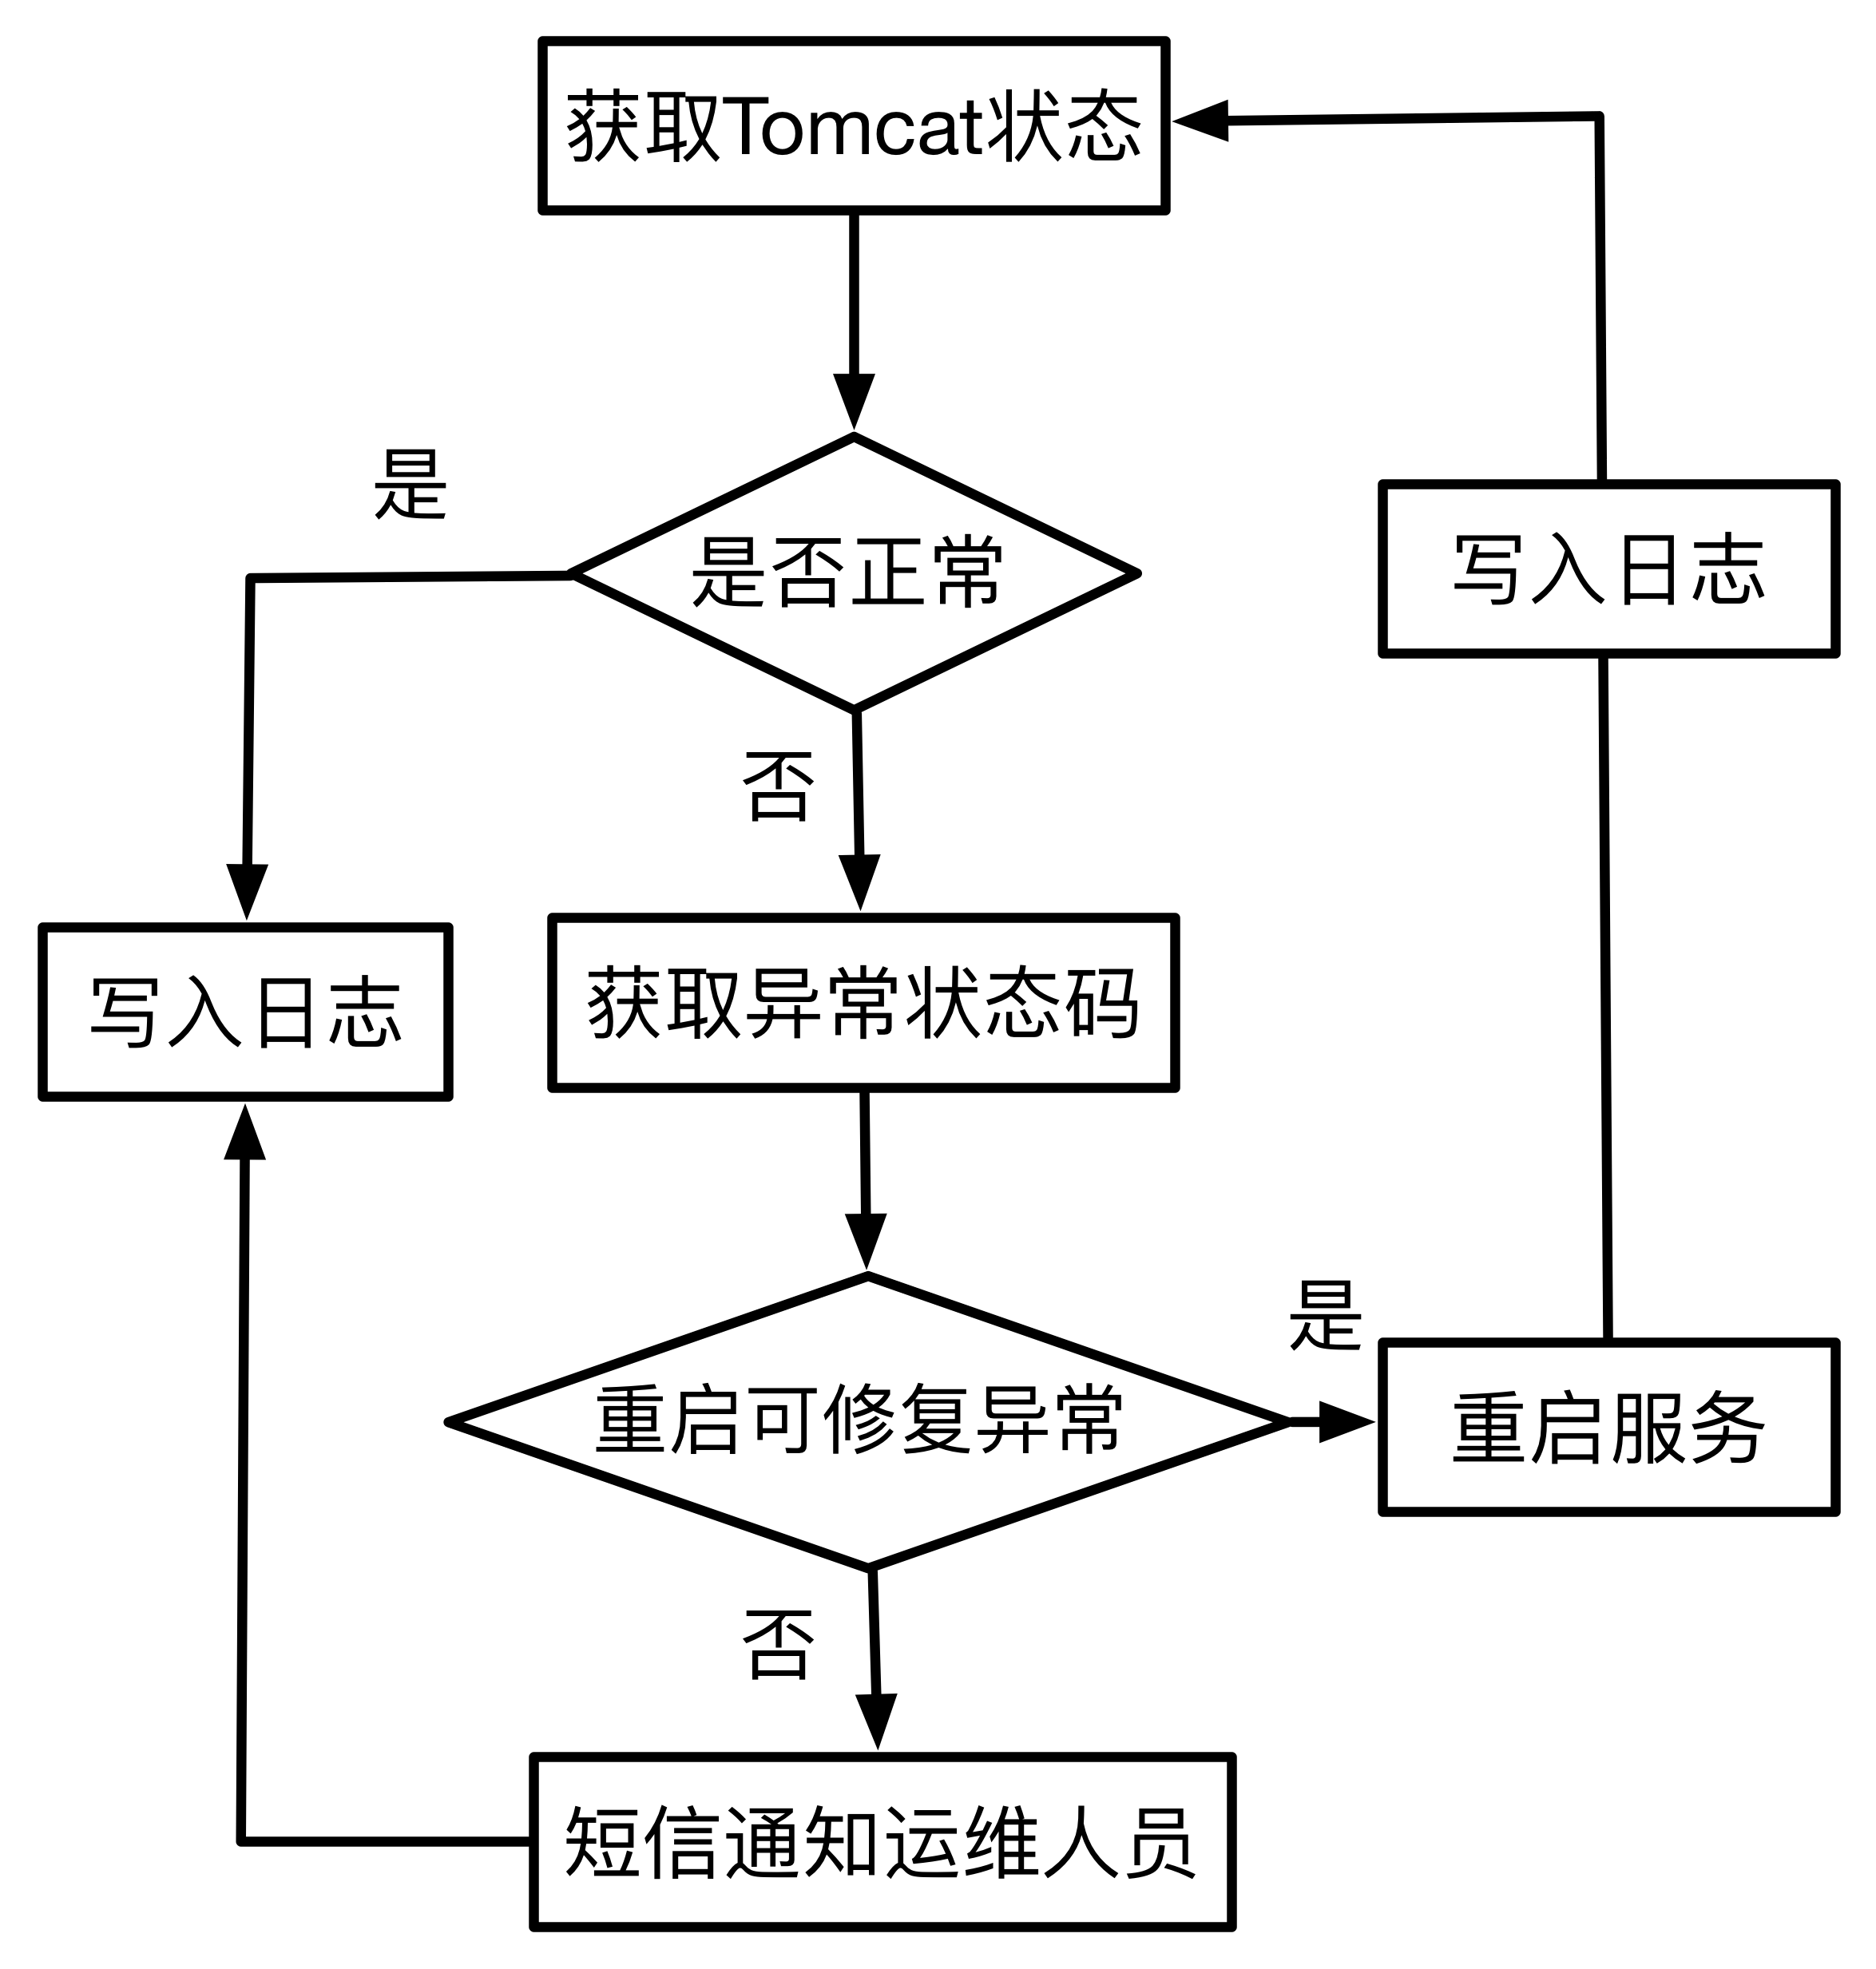
\includegraphics[height=6cm]{./img/tomcat.png}
        \caption{tomcat健康监控}
        \label{fig:mysql1}
      \end{figure}
    \end{column}
    \begin{column}{0.40\textwidth}
      \begin{block}{1. 应用监控}
        \begin{itemize}
          \item \footnotesize{为保证应用能够持续正常的提供服务,需要对所有服务器下的应用服务进行监控}
        \end{itemize}
      \end{block}
      \begin{figure}
      \centering
        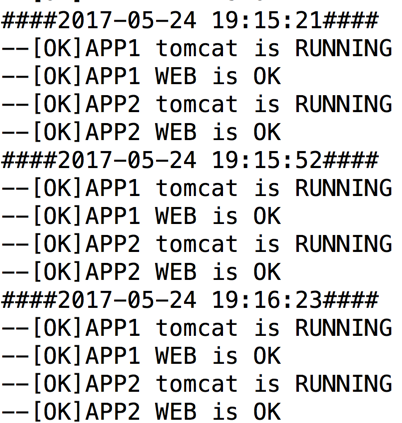
\includegraphics[height=4cm]{./img/03/tomcat1.png}
      \end{figure}
    \end{column}
  \end{columns}
\end{frame}

\begin{frame}
\frametitle{三、服务器稳定性优化}
  \begin{columns}
    \begin{column}{0.50\textwidth}
      \begin{figure}
      \centering
        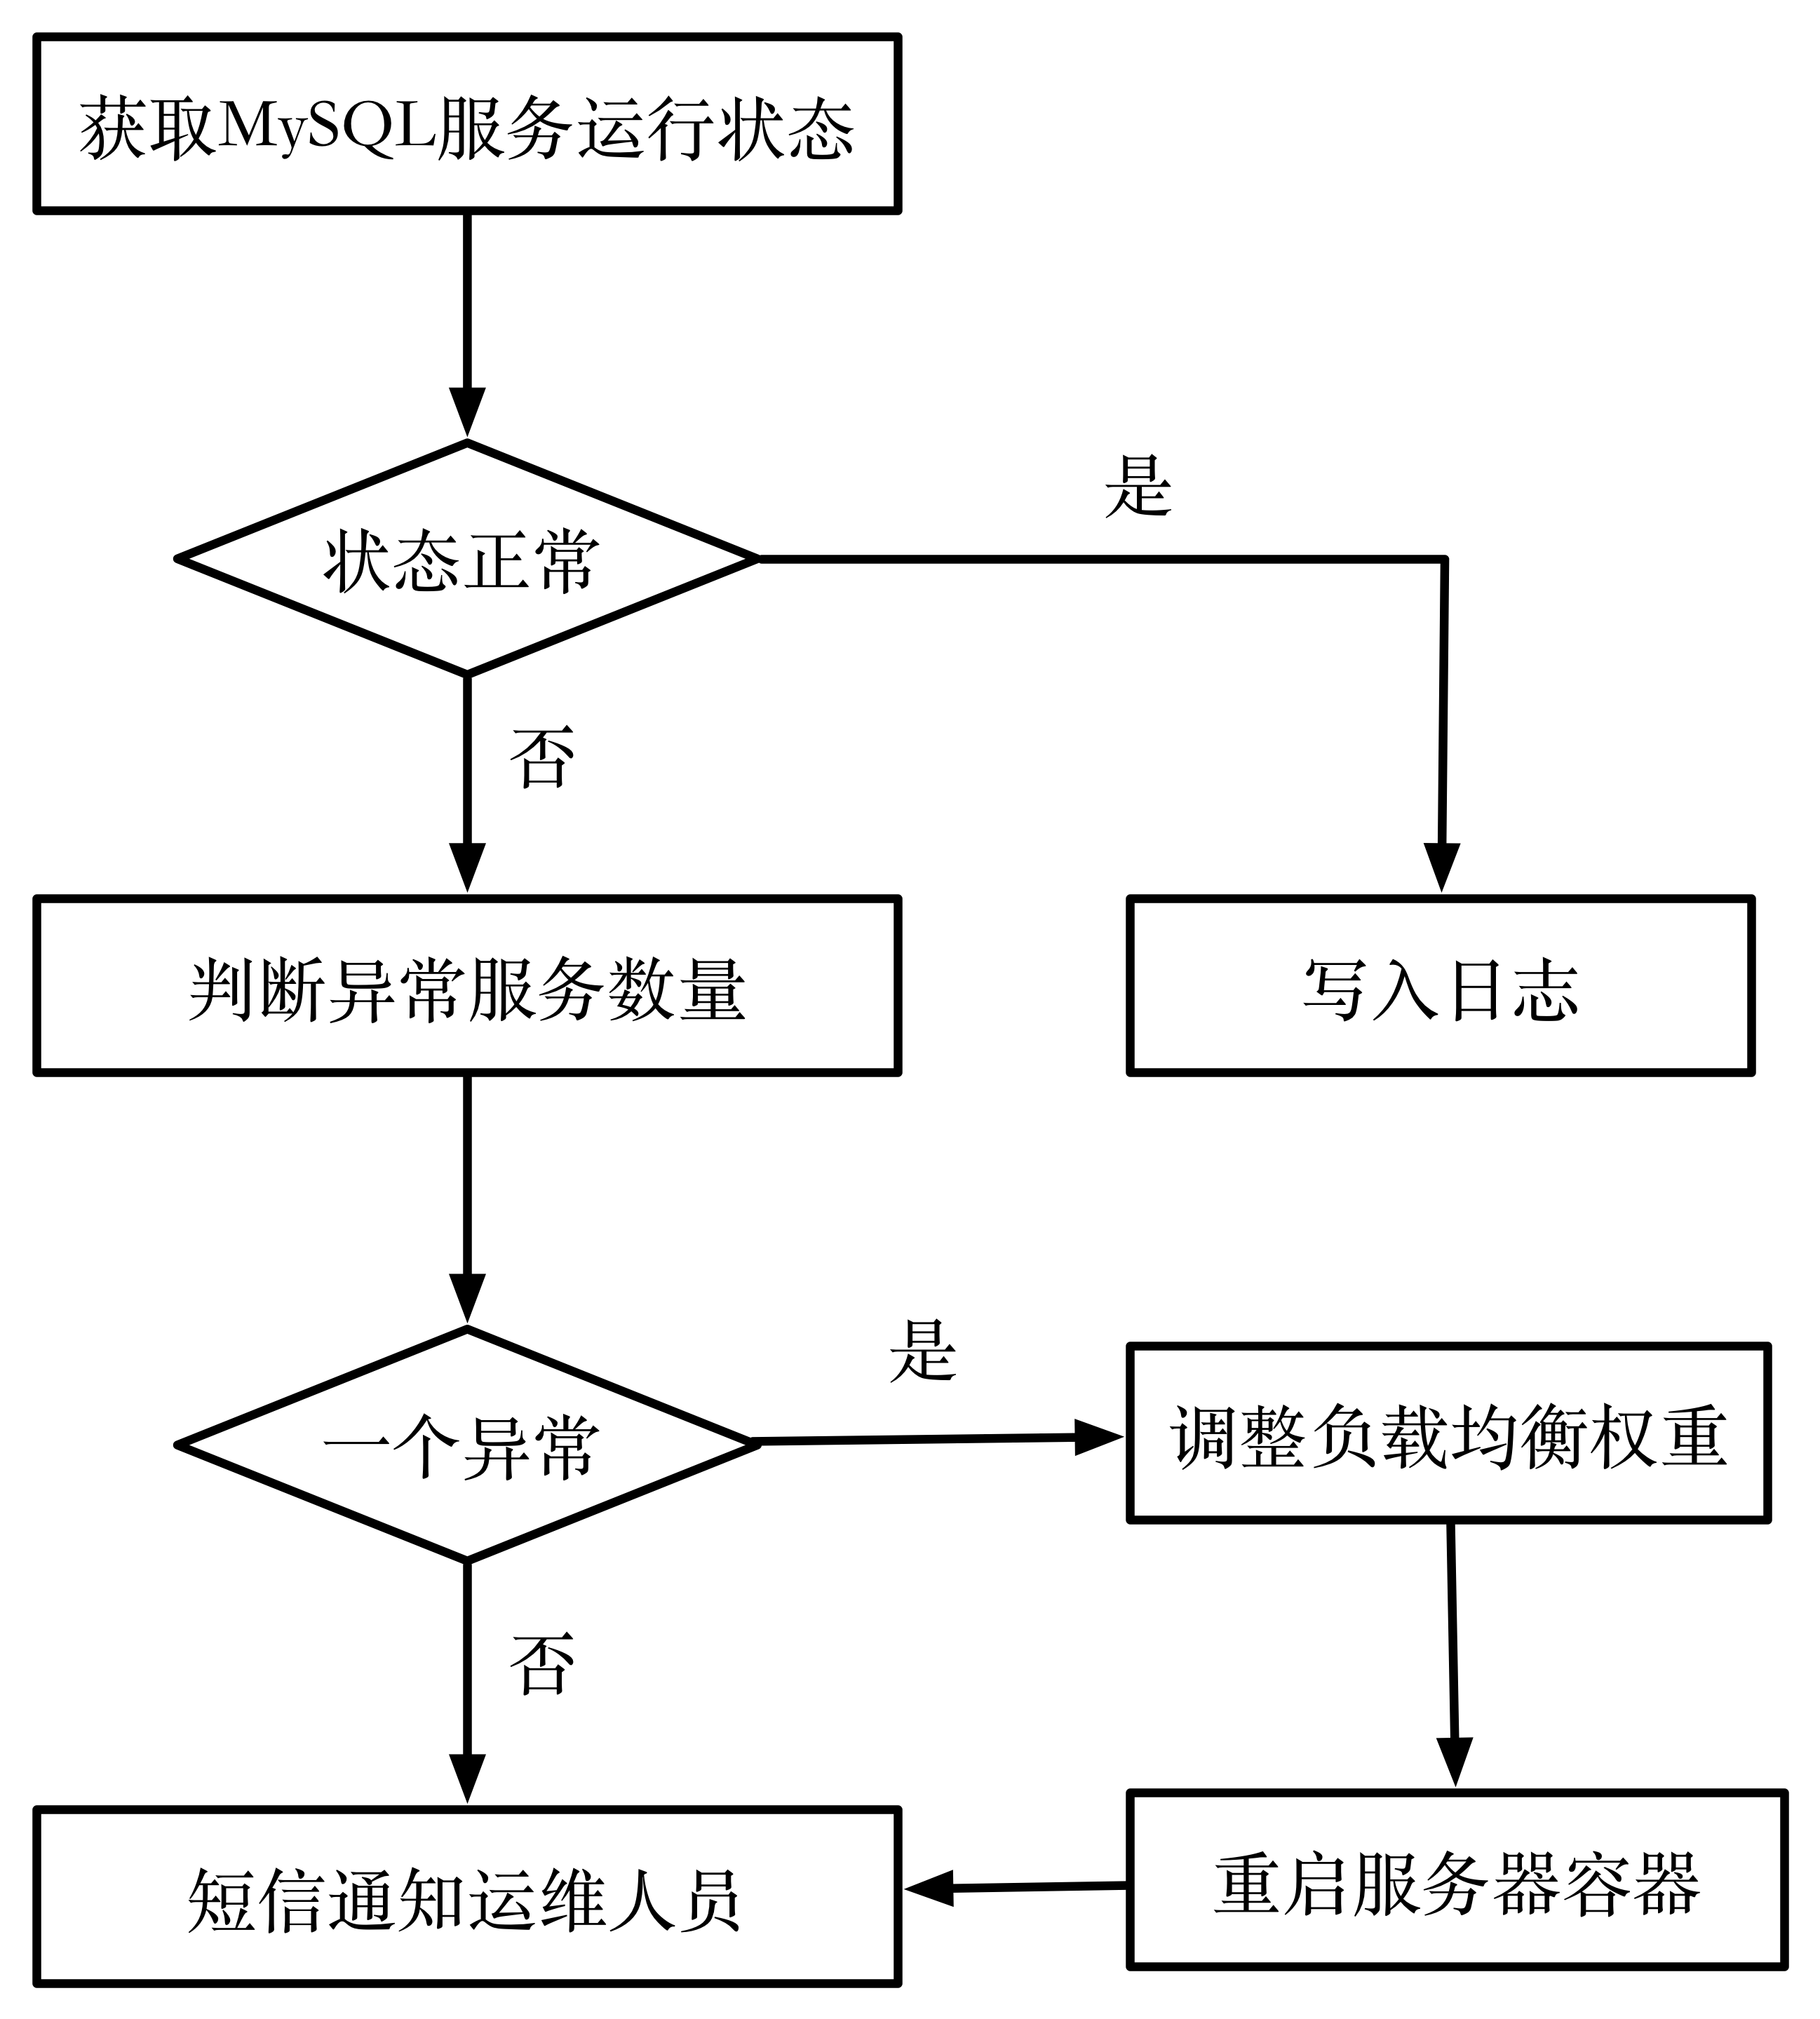
\includegraphics[height=6cm]{./img/mysql1.png}
        \caption{mysql健康监控}
        \label{fig:mysql1}
      \end{figure}
    \end{column}
    \begin{column}{0.50\textwidth}
      \begin{block}{2. 数据健康监控}
        \begin{itemize}
          \item \footnotesize{在数据库层,首先要保证的是数据库能正常提供服务,所以需要对数据库的运行状态进行监控}
        \end{itemize}
      \end{block}
      \begin{figure}
      \centering
        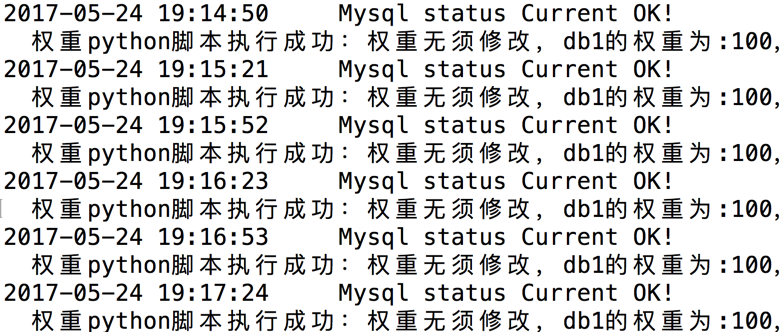
\includegraphics[height=2.5cm]{./img/03/sql1.png}
      \end{figure}
    \end{column}
  \end{columns}
\end{frame}
\begin{frame}
\frametitle{三、服务器稳定性优化}
  \begin{columns}
    \begin{column}{0.60\textwidth}
      \begin{figure}
      \centering
        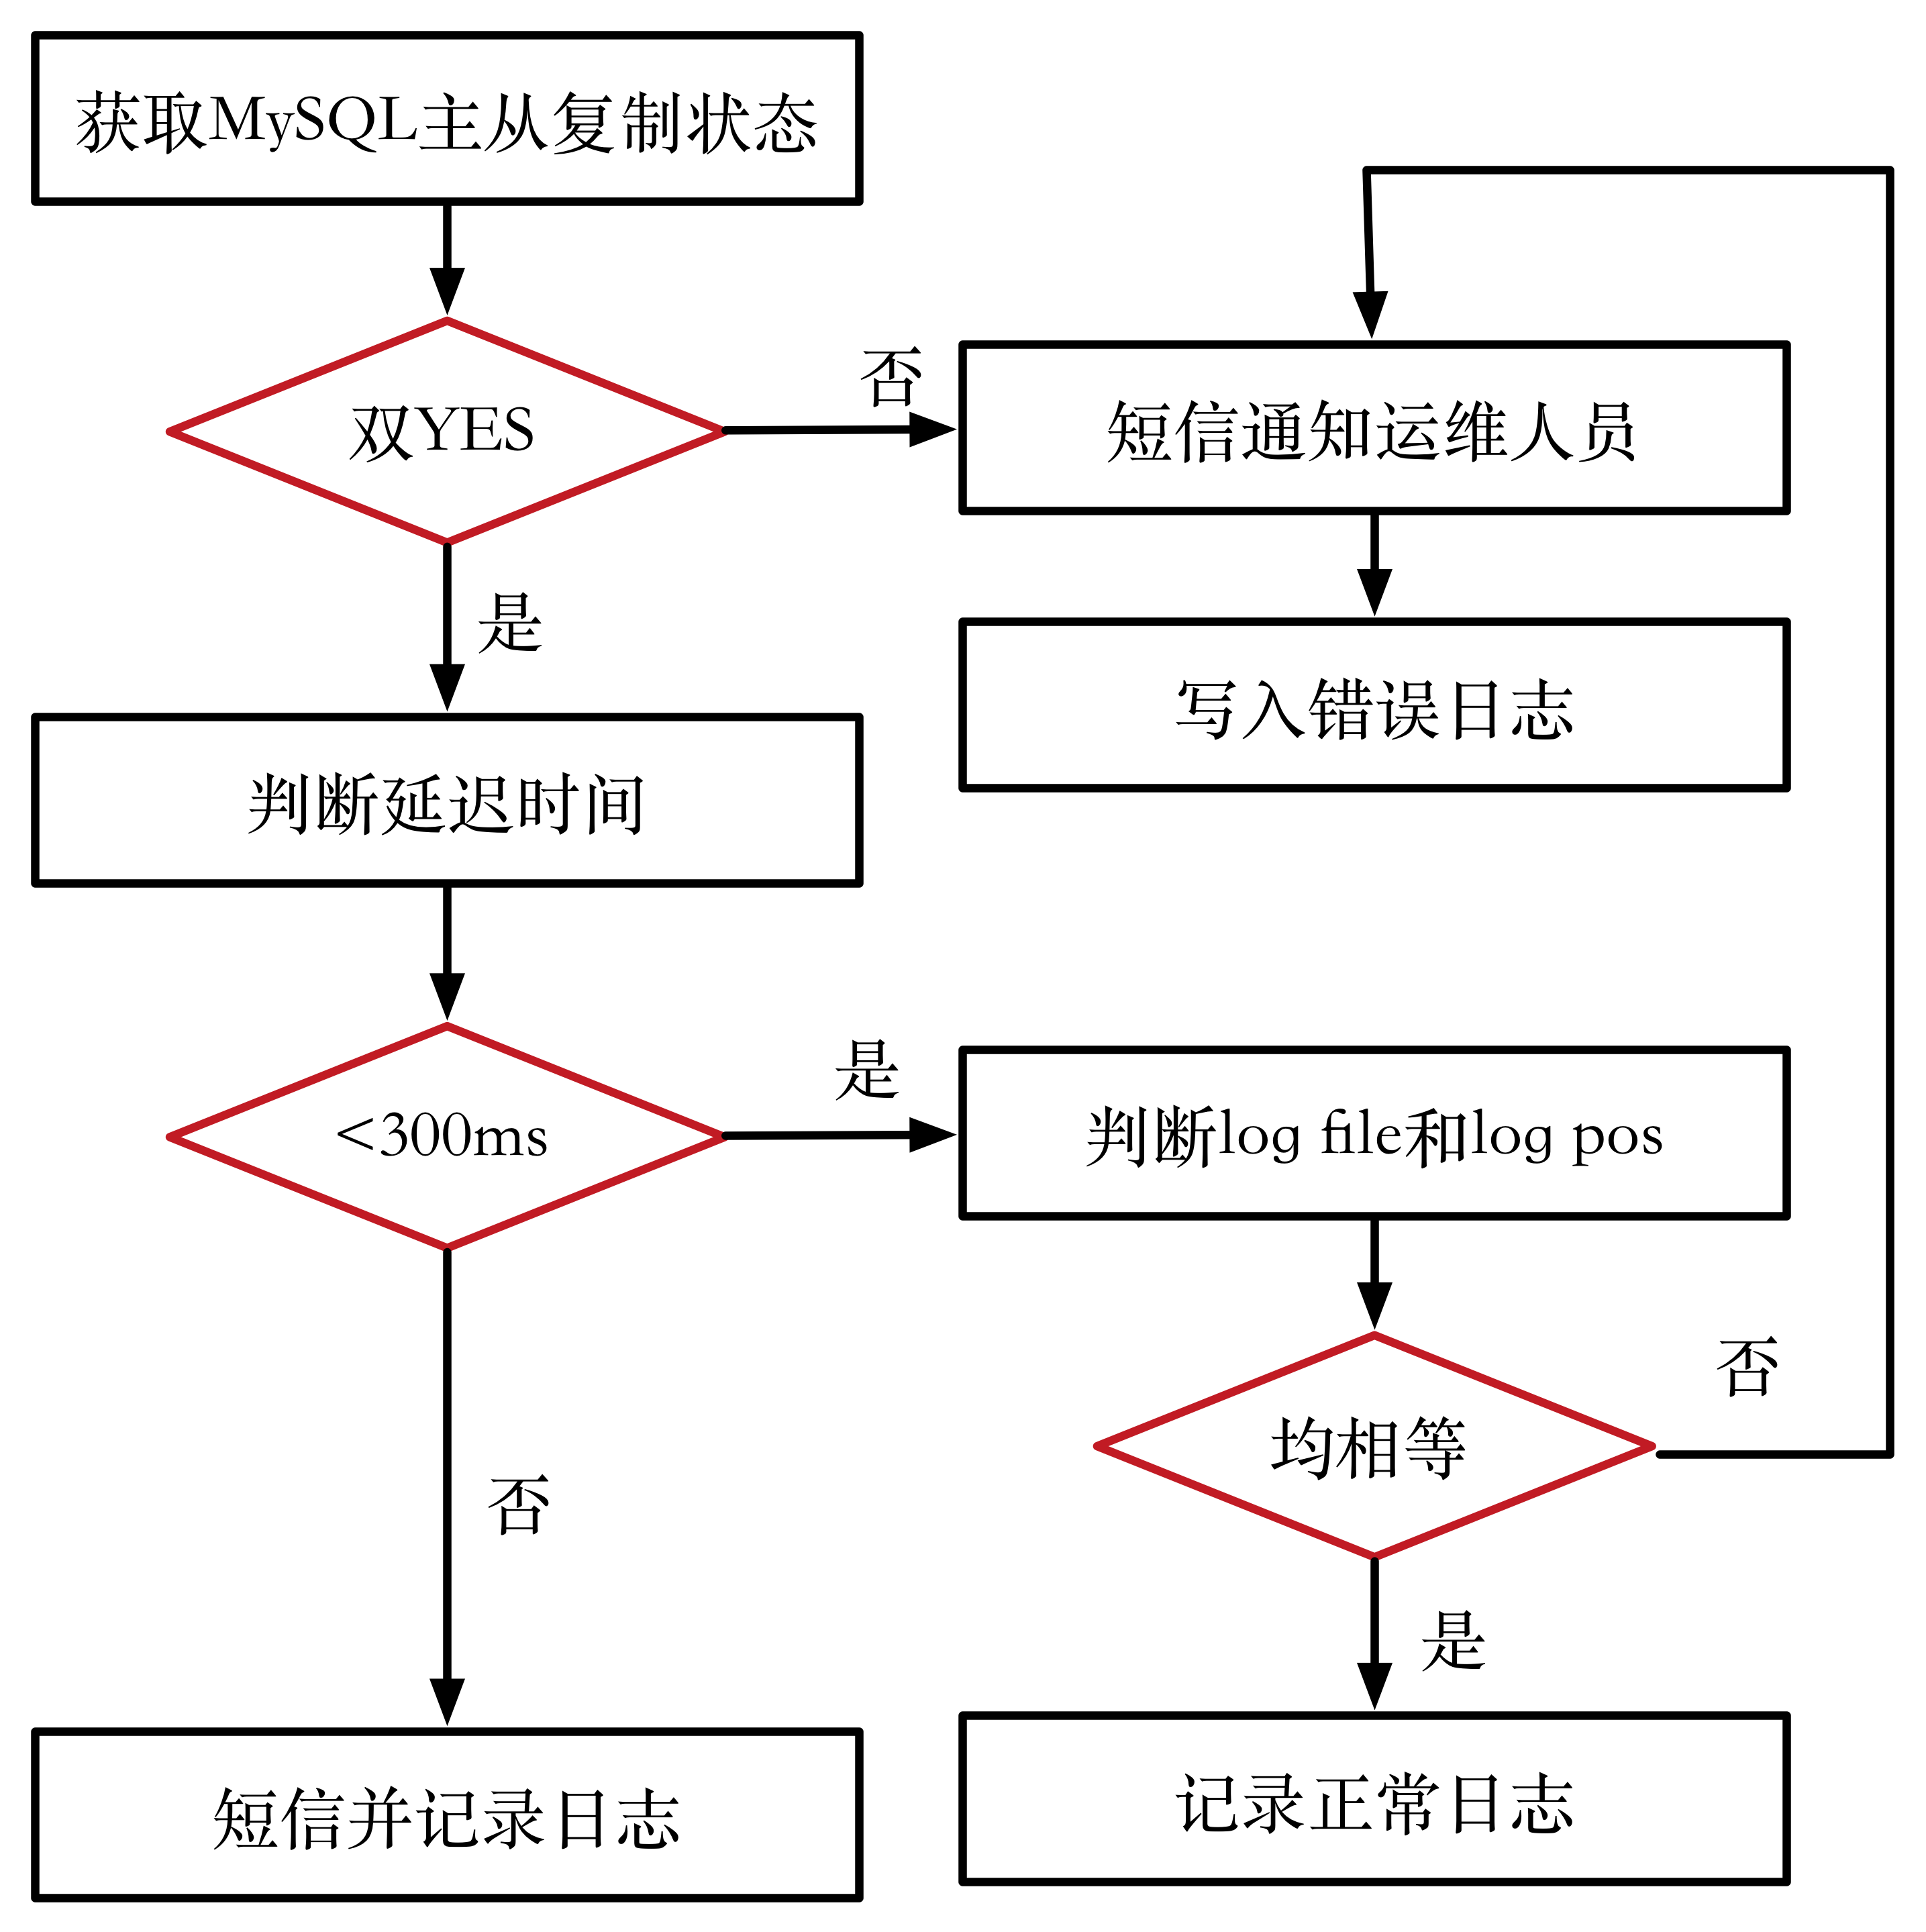
\includegraphics[height=6cm]{./img/mysql2.png}
        \caption{mysql同步监控}
        \label{fig:mysql2}
      \end{figure}
    \end{column}
    \begin{column}{0.40\textwidth}
      \begin{block}{2. 数据同步监控}
        \begin{itemize}
          \item \footnotesize{除了数据库的运行状态外,需要对数据库的主从同步状态进行监控,保证数据的完整性}
        \end{itemize}
      \end{block}
      \begin{figure}
      \centering
        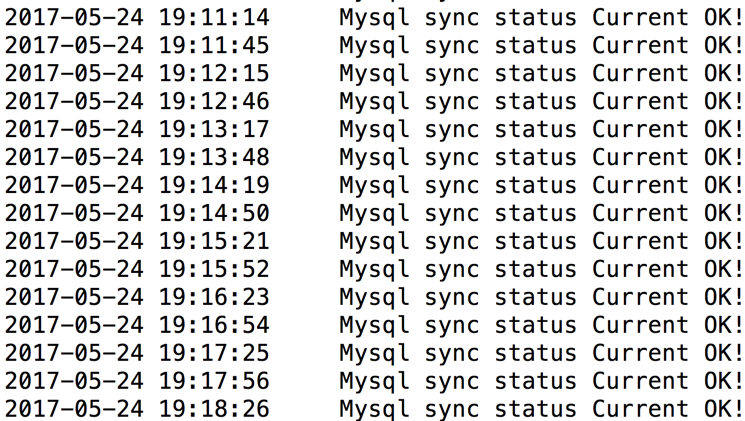
\includegraphics[height=2.5cm]{./img/03/sql2.png}
      \end{figure}
    \end{column}
  \end{columns}
\end{frame}
\begin{frame}
\frametitle{三、服务器稳定性优化}
  \begin{block}{3. 通知和备份方案设计}
    \begin{itemize}
      \item 在第一时间通知运维人员服务器状态,开发短信通知脚本;
      \item 对异常进行细致的分析,准确定位异常原因,需要对所有的监控程序进行日志的保存和备份。
    \end{itemize}
  \end{block}
  \begin{columns}
    \begin{column}{0.30\textwidth}
      \centering
      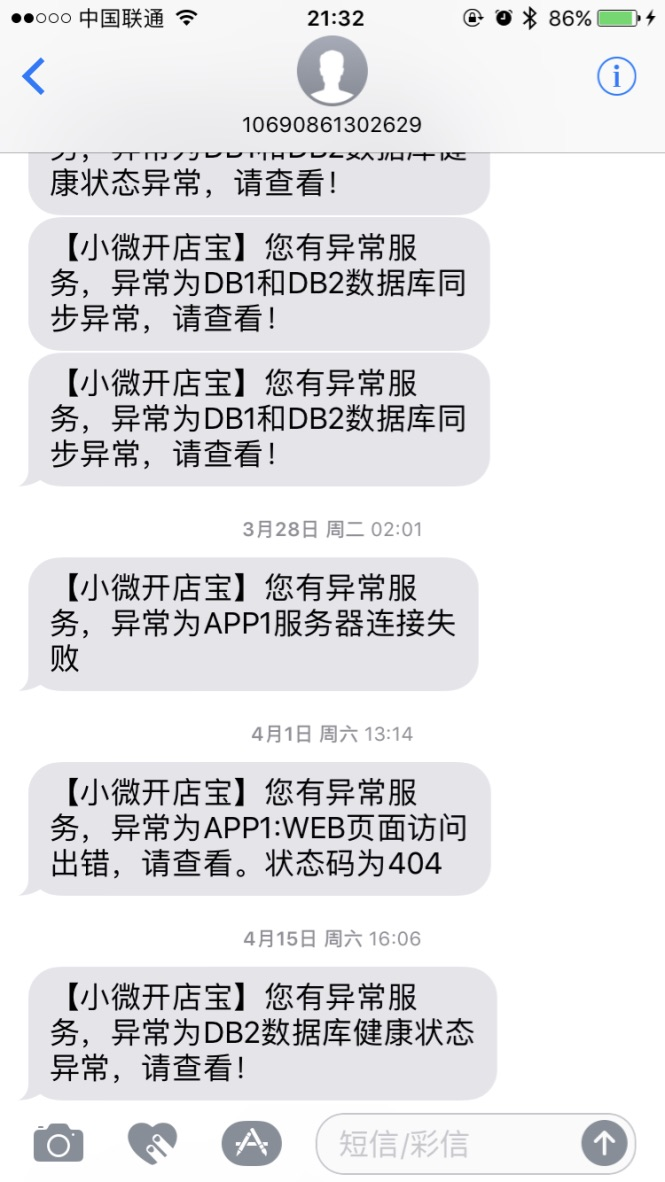
\includegraphics[height=5cm]{./img/03/message.jpg}
    \end{column}
    \begin{column}{0.70\textwidth}
      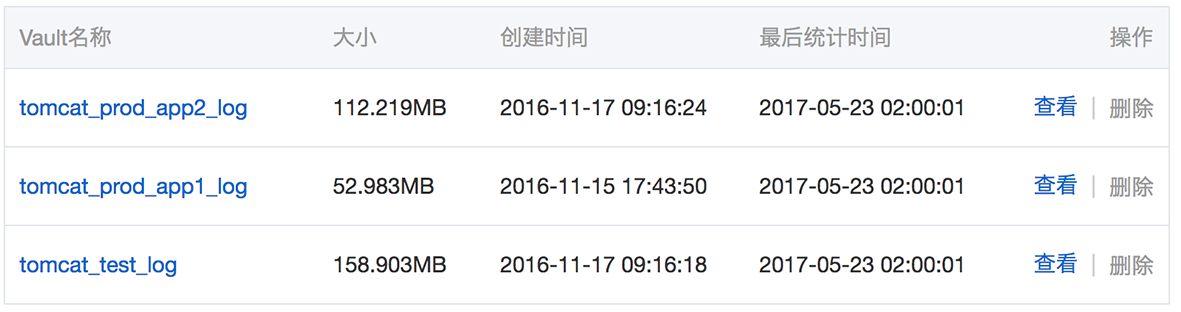
\includegraphics[height=2.5cm]{./img/03/aliyun3.png}
    \end{column}
  \end{columns}
\end{frame}
\begin{frame}
\frametitle{三、服务器稳定性优化}
   \begin{columns}
      \begin{column}{0.50\textwidth}
      	\begin{block}{4. 心跳监听开发}
	 \footnotesize{为了保证监控服务的高可用,防止服务器崩溃导致监控停止的现象发生,需要在两台服务上部署监控服务并且配置心跳监听,保证同一时间只有一台机器上的监控服务运行}
  	\end{block}
     \end{column}
     \begin{column}{0.50\textwidth}
    	 \begin{figure}
 	 \centering
   	 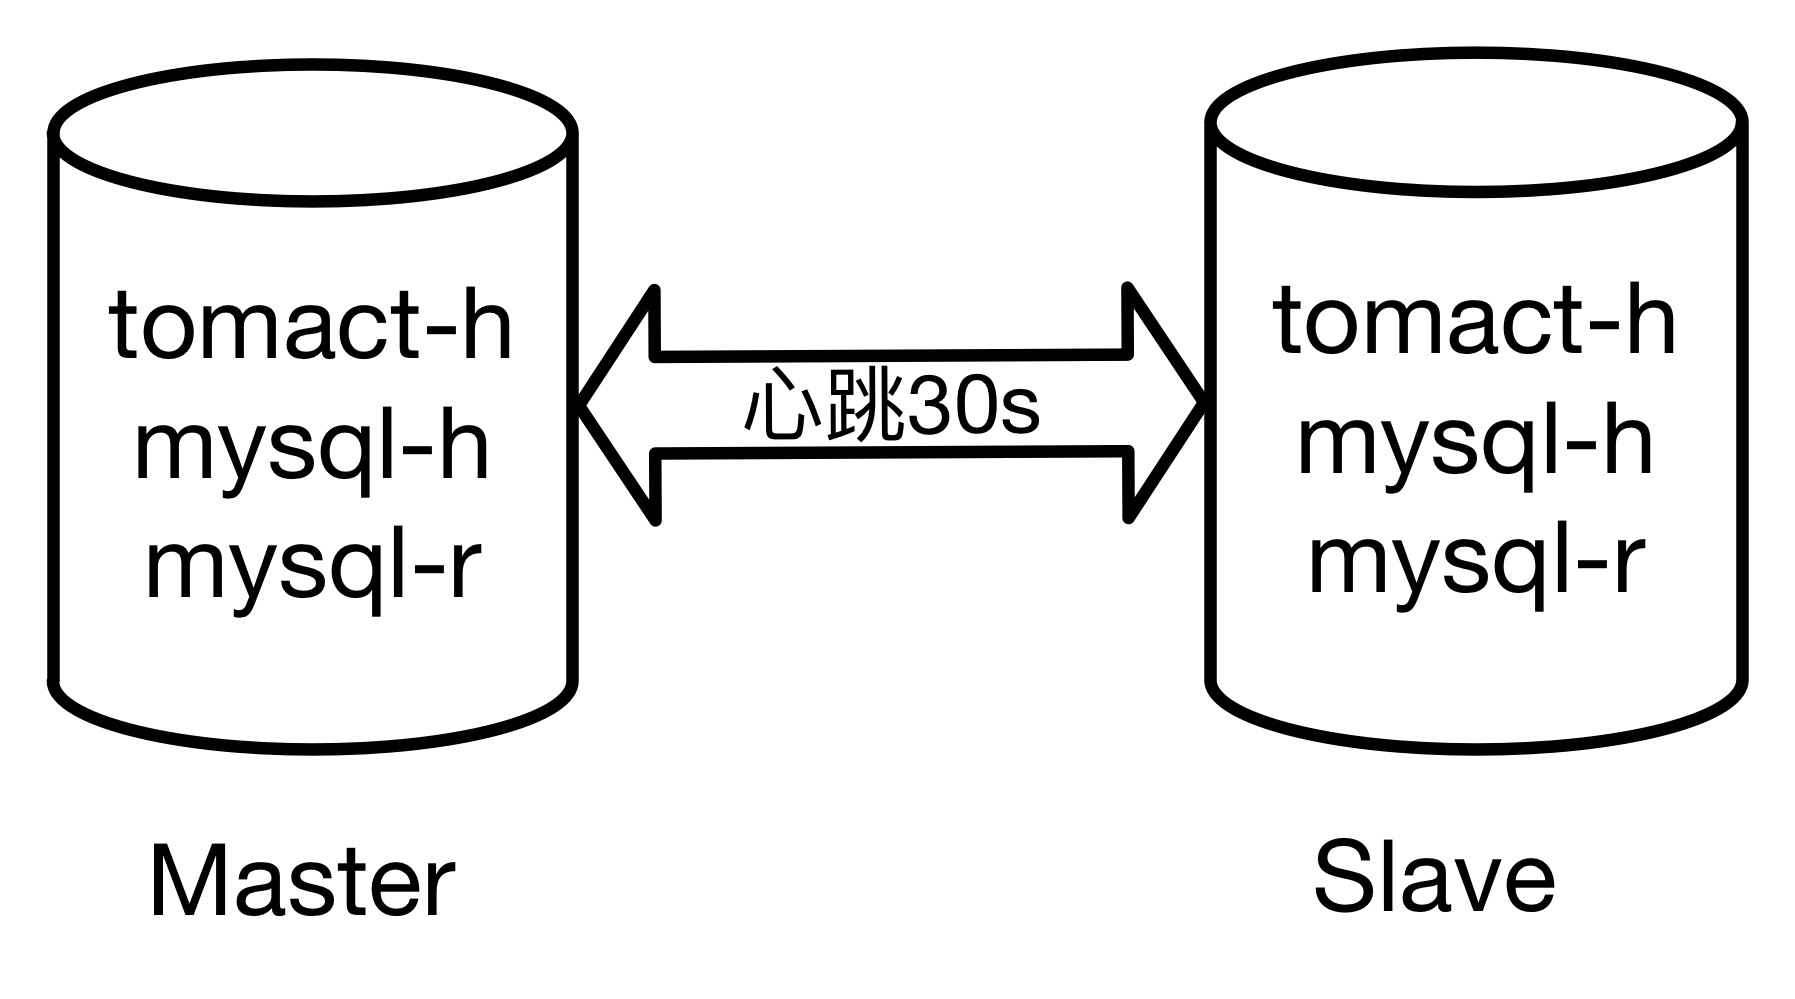
\includegraphics[height=3cm]{./img/03/ha.png}
  	\end{figure}
     \end{column}
   \end{columns}
  \begin{figure}
  \centering
    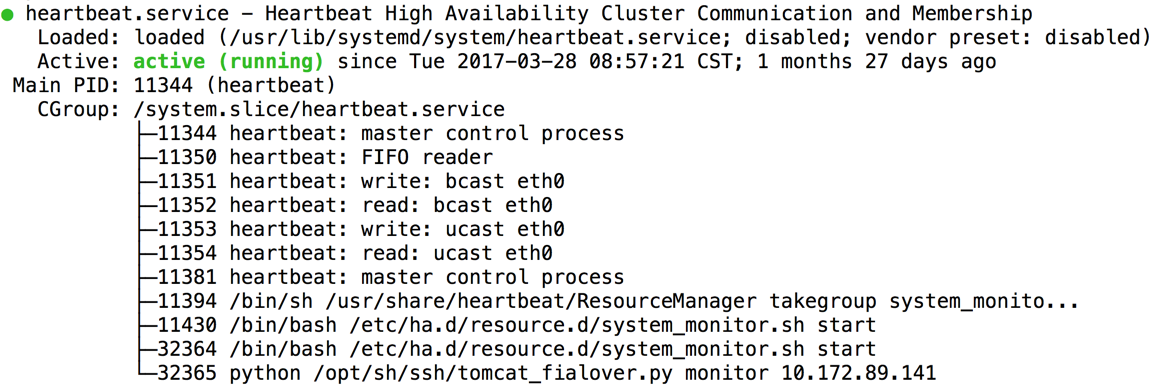
\includegraphics[height=3.5cm]{./img/ha.png}
  \end{figure}
\end{frame}
%% ++++++++++++++++++++++++++++++++++++++++++++++++++++++
%%      研究方案
%% ++++++++++++++++++++++++++++++++++++++++++++++++++++++
\begin{frame}
  \frametitle{结论及展望}
  \begin{block}{总结}
    通过应用、数据和服务器三个层级的优化策略研究,系统性能整体有了较大提升。
    \begin{enumerate}
      \item 高并发访问速度提升了21\%;
      \item 应用部署时间节省50\%;
      \item failover故障恢复时间降低至30s;
      \item 服务器节点负载均保持在85\%以下;
    \end{enumerate}
  \end{block}
  \begin{block}{展望}
  虽然通过本论文的优化,WEB 应用的性能得到了较大的提升,但是依然有很大的改进空间:
    \begin{enumerate}
      \item 探索数据库读写分离方案,从数据库的输入输出两个方面进行优化,更好的保证数据的完整性;
      \item 探索基于kubernetes的容器化集群部署方案以及监控方案;
    \end{enumerate}
  \end{block}
\end{frame}
\begin{frame}
\centering{\Huge 谢谢!}
\end{frame}

\end{document}
%% ======================================================
